% !TeX root = ../../Book2.tex
% 纲要标题：## 附录 D　叶状结构与光滑映射奇点
% 纲要位置：几何学计划纲要.md，第 2063 行。
% 正文状态：初稿；含正文、证明、例子、习题与完整解答，尚未正式审核。

% 纲要内容开始
% 
% > 以 holonomy 和喷射横截性两条明确工具链展开，不把叶空间和函数奇点视为同一分类问题。
% 
% * **叶、横截面与 holonomy**
%   * 沿叶路径的横向运输
%   * 芽群和共轭不变量
%   * 有限 holonomy 与 Reeb 局部稳定
% 
% * **叶空间与整体动力学**
%   * 环面线性叶状结构
%   * Reeb 分量及非分离叶空间
%   * Reeb 整体稳定与圆周纤维丛
% 
% * **喷射、折叠与尖点**
%   * 喷射丛和接触阶
%   * 秩分层及喷射横截
%   * 折叠与尖点的局部标准形
%   * 稳定性及维数限制
% 
% ---
% 
% 纲要内容结束

\chapter{叶状结构与光滑映射奇点}
\label{g2:app:D}
\BookChapterNumber{g2:app:D}

\begin{chapterabstract}
	叶状结构的局部坐标把流形切成平行叶片，但沿一张叶绕行后，邻近叶片可能发生非平凡的横向位移。横截面返回映射芽记录这种位移；有限 holonomy 的局部模型、环面直线叶与 Reeb 分量展示了它和叶空间拓扑的关系。对于光滑映射，喷射把指定阶数的导数组织成几何对象，横截性由此控制临界集的维数。折叠与尖点的标准形进一步说明纤维怎样合并或分开，以及这些局部形态怎样在扰动后保留。两条支线分别围绕沿叶运输与导数数据展开，最后都需要区分局部模型和整体结论。
\end{chapterabstract}

\begin{learninggoals}
	\begin{itemize}
		\item 构造沿叶路径的横向运输，核对路径复合次序，并辨认完整返回芽与线性返回映射的差别。
		\item 解释有限 holonomy 的商模型，计算附近叶的覆盖次数及叶空间，理解紧叶假设的作用。
		\item 计算环面线性叶状结构与 Reeb 分量的叶、返回映射及商拓扑，说明整体纤维丛结论需要的条件。
		\item 用喷射丛保存有限阶导数，计算矩阵秩层的余维，并通过多项式扰动理解喷射横截性。
		\item 推导折叠与平面尖点的局部标准形，计算临界值曲线和局部纤维，区分局部持续、一般位置与整体稳定。
	\end{itemize}
\end{learninggoals}

在一张叶上选一个点，再在它旁边放一张小横截面。沿叶绕一圈，怎样判断最初邻近的点是否回到了原处？第一卷第13章已经用这个问题引入横截面返回映射芽。本附录将把路径选择、同伦与坐标改变的影响逐一说明，再用这一工具比较两种看似相近的现象：紧叶附近可以是一束封闭的叶，也可以有非紧叶不断绕向它。

\ProseParagraphBreak

另一类问题从映射的临界点出发。曲面投影到平面时，投影边缘常是一条折叠曲线，曲线上还可能出现尖点。只知道微分降秩，尚不能分辨这两种形态；需要再看核方向的二阶、三阶变化。喷射把这些导数放在同一空间中，便于使用第14章的横截工具。标准形则把抽象条件变成可以画图、可以计算原像数目的公式。

\ProseParagraphBreak

叶状结构部分接第一卷第13.4节的 Frobenius 定理及第13.5节的叶空间与返回映射；光滑映射部分接本卷第14章的参数横截性、第15章的淹没与纤维丛，以及第17章的 Morse 引理。正文会在调用处提醒所需条件。有限 holonomy 的一般邻域构造、Reeb 整体稳定、光滑准备定理以及一般位置和整体稳定的指定结果，分别在使用处给出来源；局部运输、有限群模型、代表叶空间、喷射扰动和折叠、尖点的坐标计算在这里展开。

\section{叶、横截面与 holonomy}
\label{g2:sec:D01}

在一张叶状坐标图里，各张叶片看起来都是平行的；沿叶绕行一周后，附近叶片却可能错开。横截面上的返回映射把这种错开变成一个可计算的对象。本节先把返回映射的选择问题处理清楚，再解释有限返回群为何能控制一张紧叶的整个邻域。

\subsection{沿叶路径的横向运输}
\label{g2:subsec:D01:01}

本节取无边界光滑流形 \(M^{p+q}\) 上的光滑正则叶状结构 \(\mathcal F\)，叶维数为 \(p\)、余维数为 \(q\)。第一卷第13.4节的 Frobenius 定理说明，常秩对合分布能给出这样的局部坐标。我们在此使用的是定理已经得到的坐标结论：每点附近有
\[
	\varphi:U\longrightarrow B^p\times B^q,\qquad z\longmapsto(x,y),
\]
其中 \(B^p,B^q\) 是开球，连通的集合 \(y=\text{常数}\) 是\term[yepian]{叶片}[plaque]。在充分小的连通过渡区域，坐标变化具有形式
\[
	(x,y)\longmapsto\bigl(a(x,y),b(y)\bigr).
\]
第二项不依赖 \(x\)，因为它在每张连通叶片上恒定。叶由能够沿相交叶片接续的点组成，并带有这些叶片给出的流形拓扑；这项拓扑未必等于 \(M\) 的子空间拓扑。

\begin{definition}\label{g2:def:foliation-transversal-germ}
	通过 \(x\in M\) 的\term[hengjiemian]{横截面}[transversal]是一个 \(q\) 维局部嵌入子流形 \(T\)，满足
	\[
		\mathrm T_xM=\mathrm T_x\mathcal F\oplus\mathrm T_xT.
	\]
	把 \(T\) 缩小后，这个直和条件在各点成立。若两个定义在 \(x\) 的邻域上的光滑映射在某个更小邻域内相同，就说它们在 \(x\) 处有相同的\term[yingxingshunya]{映射芽}[map germ]。记局部微分同胚 \(h:(T,x)\to(T',x')\) 的芽为 \([h]_x\)。
\end{definition}

在叶状图中，横向坐标投影 \(\pi_y\) 在横截面上的微分可逆，故其限制是局部微分同胚。因此，同一张叶片内两点 \(x,x'\) 处的横截面之间有局部对应
\begin{equation}\label{g2:eq:plaque-transverse-transport}
	(\pi_y|_{T'})^{-1}\circ(\pi_y|_T).
\end{equation}
它把一点移到与它处于同一叶片的另一横截面交点。这里无需给叶选择度量，也无需规定在叶上走多快；保留下来的是叶片的接续关系。

\ProseParagraphBreak

令 \(\alpha:[0,1]\to L\) 是一张叶中的连续路径，端点为 \(x_0,x_m\)，在端点选定横截面 \(T_0,T_m\)。将区间有限细分，使每段路径落在一张叶状图的一张叶片内，在分点处另选小横截面 \(T_i\)。逐段用式\eqref{g2:eq:plaque-transverse-transport}得到 \(h_i:(T_{i-1},x_{i-1})\to(T_i,x_i)\)，再取复合
\[
	h_\alpha=h_m\circ\cdots\circ h_1.
\]
每一步只在足够小的邻域上有定义；有限次缩小起点邻域便使全部复合有定义。我们关心的是最终的芽，而不是某个任意选定的定义域。

\begin{figure}[htbp]
	\centering
	% !TeX root = ../Book2.tex
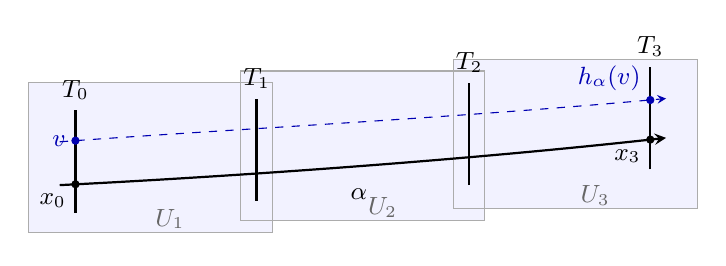
\begin{tikzpicture}[x=1cm,y=1cm,>=stealth,font=\small]
	\fill[blue!5] (0,-0.6) rectangle (3.1,1.3);
	\fill[blue!5] (2.7,-0.45) rectangle (5.8,1.45);
	\fill[blue!5] (5.4,-0.3) rectangle (8.5,1.6);
	\draw[gray!65] (0,-0.6) rectangle (3.1,1.3);
	\draw[gray!65] (2.7,-0.45) rectangle (5.8,1.45);
	\draw[gray!65] (5.4,-0.3) rectangle (8.5,1.6);
	\draw[thick,->] (0.4,0) .. controls (2.4,0.1) and (5.4,0.3) .. (8.1,0.6);
	\draw[blue!70!black,dashed,->] (0.4,0.55) .. controls (2.4,0.7) and (5.4,0.85) .. (8.1,1.1);
	\draw[thick] (0.6,-0.35)--(0.6,0.95) node[above] {\(T_0\)};
	\draw[thick] (2.9,-0.2)--(2.9,1.1) node[above] {\(T_1\)};
	\draw[thick] (5.6,0)--(5.6,1.3) node[above] {\(T_2\)};
	\draw[thick] (7.9,0.2)--(7.9,1.5) node[above] {\(T_3\)};
	\fill (0.6,0.011) circle (1.5pt) node[below left] {\(x_0\)};
	\fill[blue!70!black] (0.6,0.565) circle (1.5pt) node[left] {\(v\)};
	\fill (7.9,0.578) circle (1.5pt) node[below left] {\(x_3\)};
	\fill[blue!70!black] (7.9,1.081) circle (1.5pt) node[above left] {\(h_\alpha(v)\)};
	\node at (4.2,-0.12) {\(\alpha\)};
	\node[gray!80!black] at (1.8,-0.43) {\(U_1\)};
	\node[gray!80!black] at (4.5,-0.28) {\(U_2\)};
	\node[gray!80!black] at (7.2,-0.13) {\(U_3\)};
\end{tikzpicture}

	\caption[沿叶路径的横向运输]{沿叶路径的横向运输。实线表示所选叶上的路径，虚线表示从横截面上的邻近点出发、按相同图链接续的叶片；每一步只使用足够小的局部邻域。}
	\label{g2:fig:holonomy-transverse-transport}
\end{figure}

\begin{proposition}\label{g2:prop:holonomy-transport}
	固定端点横截面后，\([h_\alpha]_{x_0}\) 与细分、中间横截面及叶状图的选择无关，只依赖于 \(\alpha\) 在叶 \(L\) 内保持端点不动的同伦类。沿用本书先走 \(\alpha\)、再走 \(\beta\) 的路径乘法 \(\alpha*\beta\)，有
	\begin{equation}\label{g2:eq:holonomy-path-composition}
		h_{\alpha*\beta}=h_\beta\circ h_\alpha,\qquad
		h_{\alpha^{-1}}=h_\alpha^{-1},\qquad h_{\text{常路径}}=\operatorname{id},
	\end{equation}
	其中等式均为芽的等式。
\end{proposition}
\begin{proof}
	先在一张图内考虑三张横截面。记 \(p_i=\pi_y|_{T_i}\)，从第一张到第三张的直接对应为 \(p_3^{-1}p_1\)，经过第二张的对应为
	\[
		(p_3^{-1}p_2)(p_2^{-1}p_1)=p_3^{-1}p_1.
	\]
	因此插入分点和中间横截面不改变芽。若改用另一张叶状图，其横向坐标在小重叠区域满足 \(y'=b(y)\)，相应对应变成
	\[
		(b\circ p_2)^{-1}\circ(b\circ p_1)=p_2^{-1}\circ p_1.
	\]
	所以一次局部换图也不改变芽。两种覆盖路径的有限图链有共同细分：在每个分点附近缩小到两张相关图的重叠区域，并用叶内的小邻域使所用路径段都处于同一张叶片。逐段应用上述等式，再消去中间横截面的坐标变换，就得到两种构造的相同芽。有限次比较允许一次性缩小所有所需的定义域。

	再设 \(F:[0,1]^2\to L\) 是保持端点不动的同伦。对 \(L\) 使用叶自身的流形拓扑，故 \(F\) 的每一点都有一个小矩形邻域，其像落在一张叶状图的一张叶片内。紧性与 Lebesgue 数引理给出有限矩形网格，使每个小格的像都有这个性质。在网格顶点的像上选横截面；当多个顶点映到同一点时，可选同一横截面。沿一个小格的边界接续横向对应，复合为恒等芽，因为四条边都可在同一张图中计算，四次横向坐标的变换逐项消去。

	于是沿网格的一条路线，可以把某小格的两条相邻边换成另外两条，端到端的运输芽保持不变。依次越过全部小格，就把同伦下边的路线移到上边；左右两边是端点处的常路径，运输均为恒等。故上下两条路径的运输芽相同。这个论证用到有限个芽的等式，仍可在一个足够小的共同起点邻域内实现。最后，拼接两条路径的图链正好给出式\eqref{g2:eq:holonomy-path-composition}的复合次序；反向走过同一图链给出逆映射，常路径则给出恒等映射。
\end{proof}

证明中特意把同伦放在叶内：邻近叶上的点可以在 \(M\) 中很接近，却没有在同一张叶内连接它们的短路径。横向运输所保存的是指定叶中路径的变形，而不是任意环境同伦。

\subsection{芽群和共轭不变量}
\label{g2:subsec:D01:02}

闭路径的起点与终点相同，因此可以使用同一横截面。不同闭路径的返回芽组成一个群，记录附近叶片绕过这张叶时可能发生的全部局部变化。

\begin{definition}\label{g2:def:leaf-holonomy-group}
	固定 \(x\in L\) 及通过它的横截面 \(T\)。所有基于 \(x\) 的叶内闭路径所给的芽构成\term[hengjiemianfanhuinyingxingshunqun]{横截面返回映射芽群}[holonomy group]
	\[
		H(L,x,T)=\{[h_\gamma]_x:[\gamma]\in\pi_1(L,x)\}
		\subset\operatorname{Diff}_{\mathrm{germ}}(T,x).
	\]
	其中右端是固定 \(x\) 的光滑局部微分同胚芽在通常复合下构成的群。\symidx{\(H(L,x,T)\)：叶的横截面返回映射芽群}
\end{definition}

由于路径乘法先走左边，式\eqref{g2:eq:holonomy-path-composition}说明 \([\gamma]\mapsto h_\gamma\) 是反同态；也可将它看作基本群在横向芽上的右作用。若希望使用通常的左表示，则应写成
\begin{equation}\label{g2:eq:holonomy-left-representation}
	\rho:\pi_1(L,x)\longrightarrow\operatorname{Diff}_{\mathrm{germ}}(T,x),
	\qquad\rho([\gamma])=h_\gamma^{-1}.
\end{equation}
确实，\(\rho([\alpha*\beta])=h_\alpha^{-1}\circ h_\beta^{-1}=\rho([\alpha])\circ\rho([\beta])\)。两种约定得到同一个像群；此后构造群作用时采用 \(\rho\)。

\begin{proposition}\label{g2:prop:holonomy-conjugacy}
	改变横截面或在同一张叶内改变基点，所得返回芽群由横向运输共轭。因此芽群的同构类型、平凡性及有限性只依赖于叶状结构和所选的叶。
\end{proposition}
\begin{proof}
	先在同一点 \(x\) 把 \(T\) 换成 \(T'\)，以同一张叶状图内的叶片对应记作 \(c:(T,x)\to(T',x)\)。计算一条闭路径时，在起点先从 \(T'\) 返回 \(T\)，在终点再从 \(T\) 转到 \(T'\)，故新返回芽为 \(c\circ h_\gamma\circ c^{-1}\)。

	若基点从 \(x\) 移到 \(y\)，选叶内路径 \(\delta:x\to y\)，其运输为 \(h_\delta:(T_x,x)\to(T_y,y)\)。对基于 \(y\) 的闭路径 \(\gamma\)，有
	\[
		h_{\delta*\gamma*\delta^{-1}}
		=h_\delta^{-1}\circ h_\gamma\circ h_\delta.
	\]
	路径 \(\gamma\mapsto\delta*\gamma*\delta^{-1}\) 给出基本群的基点变换，故这个等式恰好给出两返回群的共轭。更换 \(\delta\) 可能改变共轭映射，却不改变“互为共轭”这一结论。
\end{proof}

在横截面上取坐标，使 \(x\) 对应于 \(0\in\mathbb R^q\)。对返回芽求微分得到
\[
	[h]_x\longmapsto\mathrm D_0h\in\operatorname{GL}(q,\mathbb R).
\]
其像称为\term[xianxinghengjiemianfanhuinqun]{线性横截面返回群}[linear holonomy group]。横截面的切空间自然映同构到法空间 \(\nu_x\mathcal F=\mathrm T_xM/\mathrm T_x\mathcal F\)，所以这项线性数据也可直接放在法空间中。换横截面时，链式法则把共轭芽变为共轭线性映射；它因而给出更容易计算的共轭不变量。

\begin{example}\label{g2:exm:parabolic-holonomy}
	在圆柱 \((\mathbb R/\mathbb Z)\times\mathbb R\) 上考虑无零点向量场
	\[
		X=\frac{\partial}{\partial\theta}+r^2\frac{\partial}{\partial r}.
	\]
	中心圆 \(L=\{r=0\}\) 是一张紧叶。取横截面 \(\theta=0\)，沿 \(\theta\) 增加一周的方向跟随邻近积分曲线，横向方程为 \(\mathrm dr/\mathrm d\theta=r^2\)。由初值 \(r(0)=s\) 解得
	\[
		r(\theta)=\frac{s}{1-\theta s},\qquad h(s)=\frac{s}{1-s}.
	\]
	对充分小的 \(s\)，解在 \(0\leq\theta\leq1\) 上存在，故这个公式确实定义返回芽。重复绕行得到
	\[
		h^n(s)=\frac{s}{1-ns},\qquad n\in\mathbb Z.
	\]
	这些芽两两不同，而 \(\mathrm D_0h^n=1\)。因此 \(H(L)\cong\mathbb Z\)，线性返回群却是平凡群。一阶导数没有看到二次项造成的累积偏移。
\end{example}

一个芽要求两个映射在某个邻域内完全一致；它比有限阶 Taylor 数据包含更多信息。\cref{g2:exm:parabolic-holonomy}说明，判断叶的稳定性时只检查线性返回群还不够。下一小节的有限性条件施加在完整的芽群上。

\subsection{有限 holonomy 与 Reeb 局部稳定}
\label{g2:subsec:D01:03}

有限芽群有一项很实用的特点：可以把各元素原先不同的定义域缩成一个共同邻域，再通过换坐标把整个群变成有限线性群。下面的平均公式同时说明这两件事。

\begin{lemma}\label{g2:lem:finite-germ-linearization}
	设 \(H\) 是固定 \(0\in\mathbb R^q\) 的光滑局部微分同胚芽的有限群。则可选取 \(0\) 的邻域及其光滑坐标，使 \(H\) 在该邻域上的代表构成实际群作用，并且在新坐标中作用为一组正交线性变换。微分映射 \(H\to\operatorname{GL}(q,\mathbb R)\) 是单射。
\end{lemma}
\begin{proof}
	对每个 \(g\in H\) 选代表 \(f_g\)，并取 \(f_e=\operatorname{id}\)。群有限，所以有限个等式 \(f_g\circ f_h=f_{gh}\) 都能在足够小的共同邻域内成立，所有需要的复合也都能在那里定义。令 \(A_g=\mathrm D_0f_g\)，则 \(A_{gh}=A_gA_h\)。在共同邻域上定义
	\[
		\Psi(y)=\frac1{|H|}\sum_{g\in H}A_g^{-1}f_g(y).
	\]
	有 \(\Psi(0)=0\) 及 \(\mathrm D_0\Psi=I\)。对每个 \(h\in H\)，把求和指标换成 \(k=gh\)，得到
	\[
		\Psi(f_h(y))
		=\frac1{|H|}\sum_{g\in H}A_g^{-1}f_{gh}(y)
		=A_h\Psi(y).
	\]
	这里先把邻域再缩小，使 \(y\) 和各 \(f_h(y)\) 都落在 \(\Psi\) 的定义域内。逆函数定理使 \(\Psi\) 在一个更小邻域上为微分同胚。

	在 \(\mathbb R^q\) 上取任意内积 \(\langle\ ,\ \rangle_0\)，再令
	\[
		\langle u,v\rangle_H=\frac1{|H|}\sum_{g\in H}\langle A_gu,A_gv\rangle_0.
	\]
	这仍是正定内积，且被全部 \(A_h\) 保持。选此内积下足够小的开球 \(B\)，使 \(\Psi^{-1}(B)\) 包含在上述各等式有效的邻域中。共轭关系说明 \(f_h\) 将 \(\Psi^{-1}(B)\) 映到自身，逆映射是 \(f_{h^{-1}}\)；这样便得到实际的群作用。在新坐标中它就是 \(A_h|_B\)。若 \(A_h=I\)，则 \(f_h\) 在这个邻域内等于恒等映射，故 \(h=e\) 作为芽也成立。
\end{proof}

现在设 \(L\) 是紧叶，\(x\in L\)，其返回芽群为有限群 \(H\)。记式\eqref{g2:eq:holonomy-left-representation}的核为 \(K\)。它是 \(\pi_1(L,x)\) 的正规子群，对应一张连通正规覆盖
\[
	\widehat L\longrightarrow L,\qquad
	\pi_1(L,x)/K\cong H.
\]
称 \(\widehat L\) 为\term[hengjiemianfanhuinfugai]{横截面返回覆盖}[holonomy cover]。这张覆盖的点可以表示为从 \(x\) 出发的叶内路径：同终点的两条路径，在它们拼成的闭路径具有恒等返回芽时识别。覆盖的层数是 \(|H|\)，所以 \(\widehat L\) 也是紧流形。

\ProseParagraphBreak

这里还需固定覆盖变换和横向作用的配合。若 \(g=\rho([\gamma])\in H\)，就在路径代表上定义 \(g[\alpha]=[\gamma*\alpha]\)。核 \(K\) 的正规性保证定义无关选择；直接计算表明这是左覆盖变换作用。横向同时用 \(g=h_\gamma^{-1}\) 作用。因此
\[
	h_{\gamma*\alpha}(h_\gamma^{-1}(v))=h_\alpha(v).
\]
这个等式说明两处作用应当同时使用：更换到同一点的路径代表时，横向起点也作相应变换，最终运输到的点才保持不变。

\begin{proposition}\label{g2:prop:finite-holonomy-model}
	设有限群 \(H\) 在连通紧流形 \(\widehat L\) 上自由光滑左作用，并在 \(\mathbb R^q\) 上忠实正交作用。取以 \(0\) 为心的开球 \(B\)，令
	\begin{equation}\label{g2:eq:finite-holonomy-model}
		E=(\widehat L\times B)/H,\qquad
		g\cdot(z,v)=(gz,gv).
	\end{equation}
	则 \(E\) 是光滑流形，乘积叶片给出叶状结构，中心叶是 \(L=\widehat L/H\)。通过 \([z,v]\) 的叶微分同胚于 \(\widehat L/H_v\)，其中 \(H_v=\{g:gv=v\}\)，其到 \(L\) 的投影是 \([H:H_v]\) 层覆盖。该叶的返回芽群同构于 \(H_v\)，叶空间同胚于 \(B/H\)。
\end{proposition}
\begin{proof}
	对角作用自由，因为任何固定 \((z,v)\) 的元素都固定 \(z\)。有限自由作用的商是流形：在 \(\widehat L\) 中取与其非平凡平移互不相交的小开集 \(V\)，则 \(V\times B\) 到商空间给出局部坐标；不同坐标之间按某个 \(g\) 改变横向坐标，仍保持乘积叶片。这也构造了 \(E\to L\) 的局部丛图。

	固定 \(v\)，映射 \(z\mapsto[z,v]\) 将 \(\widehat L\) 的像给成一张叶。两个点 \((z,v)\)、\((z',v)\) 在商中相同，当且仅当存在 \(g\in H_v\) 使 \(z'=gz\)，故这张叶为 \(\widehat L/H_v\)。它的投影到 \(\widehat L/H\) 是覆盖，纤维大小为 \(|H|/|H_v|\)。每条叶都由这种方式得到；不同的 \(v,w\) 给出同一张叶，当且仅当 \(w\in Hv\)。

	从 \((z,v)\) 出发，把商中一条闭叶内路径提升到 \(\widehat L\times B\)，提升的第二坐标保持为 \(v\)，终点为 \((gz,v)\)，其中 \(g\in H_v\)。转回起点处的横截面时，返回芽是 \(w\mapsto g^{-1}w\) 在 \(v\) 处的芽。反之，\(\widehat L\) 连通，任意 \(g\in H_v\) 都能用从 \(z\) 到 \(gz\) 的路径得到。线性作用忠实；若 \(g\) 在 \(v\) 的某邻域恒等，它就在整个向量空间恒等，因而 \(g=e\)。所以返回群确与 \(H_v\) 同构。

	最后，\([z,v]\mapsto Hv\) 是连续的开映射，其纤维恰为叶。开性可先在乘积空间用投影的开性验证，再通过有限群的开商映射下降。因此它诱导叶空间与 \(B/H\) 的同胚，而不只是集合上的双射。
\end{proof}

\begin{example}\label{g2:exm:mobius-finite-holonomy}
	取 \(\widehat L=\mathbb R/2\mathbb Z\)、\(H=\mathbb Z/2\mathbb Z\)、\(B=(-\varepsilon,\varepsilon)\)，非平凡元素作用为
	\[
		(\theta,s)\longmapsto(\theta+1,-s).
	\]
	式\eqref{g2:eq:finite-holonomy-model}给出开 Möbius 带上的圆叶状结构。中心圆的返回芽为 \(s\mapsto-s\)，返回群是二阶群；非中心圆的稳定子平凡，返回群也平凡，并且到中心圆的投影是二层覆盖。叶空间是 \([0,\varepsilon)\)，商坐标可取 \(|s|\)。每张叶都是圆，却不能把这个叶状邻域写成保持中心叶的 \(S^1\times(-\varepsilon,\varepsilon)\) 乘积，因为乘积的中心叶返回群平凡，而返回群在叶状微分同胚下保持共轭类型。
\end{example}

一般叶状结构中，紧叶附近是否一定有上述模型，是 Reeb 局部稳定定理所回答的问题。名称中的 Reeb 指法国数学家 Georges Reeb。\footnote{Georges Reeb（1920--1993），法国数学家，研究微分拓扑、叶状结构与动力系统。}

\begin{theorem}[Reeb 局部稳定定理]\label{g2:thm:reeb-local-stability}
	设 \(\mathcal F\) 是无边界光滑流形 \(M\) 上的光滑正则叶状结构，\(L\) 是紧叶，完整的横截面返回映射芽群 \(H\) 有限。则 \(L\) 有任意小的开\term[baoheneiyu]{饱和邻域}[saturated neighborhood]，即由完整叶组成的开邻域 \(U\)，使 \((U,\mathcal F|_U)\) 与式\eqref{g2:eq:finite-holonomy-model}的叶状模型微分同胚，并将 \(L\) 对应到中心叶。这里 \(\widehat L\) 是横截面返回覆盖，\(H\) 在横向开球上的作用取自其线性化。特别地，\(U\) 中的每张叶都紧，且具有有限返回芽群。
\end{theorem}
\begin{proof}
	本证明使用如下邻域存在性结果：若一张叶 \(S\) 嵌入且具有有限返回芽群，则 \(S\) 在原流形中的某开邻域，与其模型 \((\widehat S\times\nu_x\mathcal F)/H\) 中零叶的某开邻域叶状微分同胚，并在零叶上为给定识别。这一结果允许 \(S\) 非紧，给出的邻域此时不要求饱和；其一般证明见\cite[第2节，引理1，222--226页]{CrainicMarcut2015ReebStability}。下面完整说明紧性怎样把这项邻域结论变成定理所需的饱和模型。

	紧叶 \(L\) 的包含是从紧流形到 Hausdorff 流形的单射浸入，故为嵌入，可以应用上述结果。记所得叶状微分同胚为 \(F:W\to V\)，其中 \(W\) 是模型零叶的开邻域，\(V\subset M\) 是开邻域。有限芽群由\cref{g2:lem:finite-germ-linearization}线性化，并选好不变内积。\(\widehat L\) 是紧流形，故 \(W\) 在 \(\widehat L\times\nu_x\mathcal F\) 中的原像包含 \(\widehat L\times B\)，其中 \(B\) 是充分小的不变开球。这一步可从 \(\widehat L\times\{0\}\) 的有限乘积邻域子覆盖直接得到。

	令 \(U=F((\widehat L\times B)/H)\)。这是 \(M\) 的开子集。由\cref{g2:prop:finite-holonomy-model}，模型中的每张叶 \(N=\widehat L/H_v\) 都紧。其像包含于原叶状结构的一张叶 \(L'\)；叶状局部坐标说明 \(F|_N:N\to L'\) 对叶自身的拓扑光滑，并且局部微分同胚，所以像在 \(L'\) 中开。这个像又是紧集，而 \(L'\) 是 Hausdorff 流形，故像在 \(L'\) 中闭。叶 \(L'\) 连通，像非空，因此像就是整张 \(L'\)。这就证明 \(U\) 饱和；邻近叶的紧性和有限返回群也由模型命题得到。

	若另给 \(L\) 的任意环境开邻域 \(O\)，在模型中把 \(W\) 换成 \(W\cap F^{-1}(O\cap V)\)，仍是紧零叶的开邻域。重复刚才有限子覆盖的选择，将 \(B\) 缩小便得到 \(U\subset O\)。故这种饱和邻域确实可以任意小。
\end{proof}

\begin{corollary}\label{g2:cor:trivial-holonomy-product}
	若紧叶 \(L\) 的返回芽群平凡，则存在任意小的饱和邻域，叶状微分同胚于 \(L\times B^q\)，各叶对应于 \(L\times\{v\}\)。若余维为 \(1\)，且叶状结构在 \(L\) 附近横向可定向，则有限返回芽群必平凡，因而同样得到这种乘积邻域。
\end{corollary}
\begin{proof}
	当 \(H\) 平凡时，\(K=\pi_1(L,x)\)，相应的覆盖就是 \(\widehat L=L\)，所以模型直接化为乘积。在余维一且横向可定向时，各返回芽保持横向定向，其导数为正数。有限群中的每个导数都有有限乘法阶，正实数中具有有限阶的元素只有 \(1\)。\cref{g2:lem:finite-germ-linearization}的单射性于是给出 \(H=\{e\}\)。
\end{proof}

定理的局部范围是整张紧叶的邻域，因此比单点处的叶状坐标强得多。紧性保证能统一选择横向宽度，并把模型中的紧叶识别为环境中的完整叶；有限芽群保证全部返回可以同时控制。\cref{g2:exm:parabolic-holonomy}虽有紧叶和平凡线性返回群，却有无限的完整芽群，因而不能从它推出上述饱和乘积结论。下一节将直接观察这种局部返回行为如何影响叶空间。

\section{叶空间与整体动力学}
\label{g2:sec:D02}

横截面上的返回映射描述邻近叶怎样绕行；把整条叶压成一点，得到的商空间则记录不同叶能否分开。局部坐标盒总像一叠平行切片，商空间却可能是圆周，也可能连不同点都无法用开集区分。本节从环面上可以显式求解的流出发，再构造一个紧叶与非紧叶共存的实心环面。

\subsection{环面线性叶状结构}
\label{g2:subsec:D02:01}

令 \(T^2=\mathbb R^2/\mathbb Z^2\)，在上面取处处非零的向量场
\[
	X_\alpha=\partial_x+\alpha\partial_y,\qquad \alpha\in\mathbb R.
\]
它的叶由轨道 \(t\mapsto[x_0+t,y_0+\alpha t]\) 给出。这也是闭一形式 \(\mathrm dy-\alpha\mathrm dx\) 的核所确定的叶状结构。第一卷第13.5节已证明有理斜率的叶闭合、无理斜率的叶稠密；这里恢复计算，并把结果与叶空间及 holonomy 联系起来。

\begin{definition}\label{g2:def:foliation-leaf-space}
	设 \(\mathcal F\) 是光滑流形 \(M\) 上的叶状结构。将同一叶内的点识别所得集合 \(M/\mathcal F\)，赋予商映射 \(q:M\to M/\mathcal F\) 所确定的商拓扑，称为\term[yekongjian]{叶空间}[leaf space]。由整条叶组成的子集称为\term[baoheji]{饱和集}[saturated set]；商中的开集恰对应 \(M\) 中的饱和开集。
\end{definition}

\begin{proposition}\label{g2:prop:torus-foliation-quotient}
	对上述 \(T^2\) 上的光滑线性叶状结构，有以下结论。
	\begin{enumerate}
		\item 若 \(\alpha=p/q\)，其中 \(p,q\) 互素且 \(q>0\)，则每条叶为嵌入圆周，最小正流周期为 \(q\)。映射 \([x,y]\mapsto[qy-px]\) 将叶空间微分同胚地识别为圆周，并给出以这些叶为纤维的光滑纤维丛。
		\item 若 \(\alpha\) 无理，则每条叶自身微分同胚于 \(\mathbb R\)，其像在 \(T^2\) 中稠密。叶空间有不止一个点，但其开集只有空集与全空间。
		\item 两种情形中，每条叶的 holonomy 群都平凡。
	\end{enumerate}
\end{proposition}
\begin{proof}
	轨道在时刻 \(t\) 回到初始点，当且仅当 \(t\in\mathbb Z\) 且 \(\alpha t\in\mathbb Z\)。有理情形的返回时间正是 \(q\mathbb Z\)，所以轨道是紧圆周的单射浸入，因而是嵌入。令 \(P([x,y])=[qy-px]\)。其微分为处处非零的 \(q\mathrm dy-p\mathrm dx\)，且沿叶为零。若两点的 \(P\) 值相同，则对实代表有 \(q\Delta y-p\Delta x=k\in\mathbb Z\)。由互素性选整数 \(m,n\) 使 \(qn-pm=k\)，于是 \((\Delta x-m,\Delta y-n)\) 沿方向 \((q,p)\)。这说明它们恰在同一条叶上。

	映射 \(P\) 是满淹没，源紧，故由\cref{g2:thm:ehresmann}成为光滑纤维丛。其局部投影坐标给商空间赋予圆周的光滑结构。也可以先看拓扑：它诱导从紧叶空间到 Hausdorff 圆周的连续双射，因而是同胚。

	无理情形没有非零返回时间，轨道在叶自身的流形结构下以 \(\mathbb R\) 参数化。为恢复稠密性的理由，将 \(0,\alpha,\ldots,N\alpha\) 的小数部分放入 \(N\) 个等长区间；两数之差及其适当正负号给出
	\[
		0<\delta=k\alpha-m<1/N
	\]
	其中 \(k,m\) 为整数。模 \(1\) 的整数倍 \(\alpha\) 因而包含步长小于 \(1/N\) 的一组网点，随 \(N\) 增大可任意逼近圆周上的点。对环面中任意开矩形，先选其中第一坐标 \(u\)，再考察时刻 \(u-x_0+n\)；第二坐标的取值是一个无理旋转轨道，必能进入该矩形。故每条叶稠密。

	每条叶在截面 \(x=0\) 上只交于可数多个点，而该截面不可数，所以不止一条叶。若 \(U\) 是非空饱和开集，每条稠密叶都与 \(U\) 相交，饱和性又使它整条包含于 \(U\)，所以 \(U=T^2\)。这给出第二项的商拓扑。

	截面 \(x=0\) 的首次正返回映射为 \(R_\alpha([y])=[y+\alpha]\)。有理情形中，沿完整闭叶一周对应 \(R_\alpha^q=\mathrm{id}\)，故 holonomy 平凡。无理情形的叶为 \(\mathbb R\)，其全部叶内环路可缩；由\cref{g2:prop:holonomy-transport}的同伦不变性，holonomy 也平凡。
\end{proof}

无理斜率的首次返回映射确实在不断移动截面上的点，但这些运动没有沿叶内环路回到原来的叶内基点。这说明返回轨道的稠密性与环路芽群是两种信息。叶的自身拓扑也必须保留：能选 \(|n_j|\to\infty\) 使 \(n_j\alpha\bmod1\to0\)，于是轨道像在环境中趋回出发点，而叶内参数并未趋回零。因此无理叶到环面的单射浸入不是嵌入。

\ProseParagraphBreak

这个例子还显示一种整体不稳定性。若 \(\alpha_j\to\alpha\)，对应线分布在 \(C^\infty\) 意义下收敛；常系数的各阶导数没有额外误差。可是有理数与无理数都在实数中稠密，任意小的斜率改变都可能把全部圆周叶换成稠密直线叶。微分同胚保持叶的紧性，因而这两类叶状结构不可能通过保持叶的微分同胚等同。

\subsection{Reeb 分量及非分离叶空间}
\label{g2:subsec:D02:02}

现在希望让一张紧叶成为其他叶的极限。取实心环面
\[
	V=D^2\times(\mathbb R/\mathbb Z),\qquad
	D^2=\{(x,y):x^2+y^2\le1\},\qquad \rho=x^2+y^2,
\]
纵向圆坐标记为 \(t\)。角坐标 \(t\) 在实值意义下只局部定义，但 \(\mathrm dt\) 是全局一形式。考虑
\begin{equation}\label{g2:eq:reeb-solid-torus-form}
	\alpha=\mathrm d\rho+(1-\rho)\mathrm dt.
\end{equation}
在中心圆 \(\rho=0\) 上，它等于 \(\mathrm dt\)；在 \(\rho>0\) 处，径向分量 \(\mathrm d\rho\) 非零。因此 \(\alpha\) 处处非零，其核是一张光滑二维分布。

\ProseParagraphBreak

直接计算得到 \(\mathrm d\alpha=-\mathrm d\rho\wedge\mathrm dt\)，从而 \(\alpha\wedge\mathrm d\alpha=0\)。这个等式说明核分布对合：若 \(X,Y\) 都在核中，外微分公式给出 \(\alpha([X,Y])=-\mathrm d\alpha(X,Y)=0\)。最后一个等式也可由取 \(\alpha(Z)=1\) 后在 \((Z,X,Y)\) 上计算 \(\alpha\wedge\mathrm d\alpha\) 得到。第一卷第13.4节的 Frobenius 定理于是适用。在边界附近，将同一公式延伸到 \(\rho>1\) 的小领圈，仍为非零可积形式，所以边界处的叶状结构也由通常无边流形上的局部定理限制而来。

\begin{proposition}\label{g2:prop:reeb-component-leaves}
	式\eqref{g2:eq:reeb-solid-torus-form}在实心环面上确定的叶状结构有一张边界环面叶 \(L_\partial=\partial D^2\times S^1\)。全部内部叶以 \(c\in\mathbb R/\mathbb Z\) 编号，表达为
	\begin{equation}\label{g2:eq:reeb-plane-leaves}
		L_c=\{(z,t):|z|<1,\ t=c+\log(1-|z|^2)\pmod1\}.
	\end{equation}
	每条 \(L_c\) 是嵌入开圆盘，且在 \(V\) 中的闭包为 \(L_c\cup L_\partial\)。沿边界叶的子午圈，单侧 holonomy 为恒等；沿正向纵圈，以向内坐标 \(s=1-\rho\) 表示的返回芽为 \(s\mapsto e s\)。
\end{proposition}
\begin{proof}
	在 \(\rho=1\) 上，\(\alpha=\mathrm d\rho\)，其核恰是边界切空间，所以整个连通边界为一张叶。在内部，令
	\[
		F(z,t)=t-\log(1-|z|^2)\pmod1.
	\]
	则 \(\mathrm dF=\alpha/(1-\rho)\)。每个纤维由式\eqref{g2:eq:reeb-plane-leaves}给出，是开圆盘上的光滑图像；投影到 \(z\) 是其光滑逆，所以它连通且嵌入。由于 \(F\) 是淹没，这些纤维正是内部的最大叶。

	固定边界点 \((e^{i\varphi},t_0)\)。选实代表 \(c,t_0\)，令
	\[
		r_k^2=1-\exp(t_0-c-k).
	\]
	当 \(k\) 充分大时，\(0<r_k<1\)，并且 \((r_ke^{i\varphi},t_0)\in L_c\)，趋向所选边界点。这证明边界全部包含于闭包；内部的其余纤维由连续的 \(F\) 分开，不会增加其他内部极限点。

	沿子午圈只改变极角 \(\varphi\)，\(\rho,t\) 均不变，故横向点原样返回。沿纵圈令 \(t\) 从 \(0\) 增至 \(1\)，保持极角不变；要切于叶，必须满足
	\[
		\frac{\mathrm d\rho}{\mathrm dt}=-(1-\rho),\qquad
		\frac{\mathrm ds}{\mathrm dt}=s.
	\]
	因此 \(s(1)=e s(0)\)。将初始 \(s\) 限于足够小邻域，就能走完整个纵圈。反向纵圈则给出收缩芽 \(s\mapsto e^{-1}s\)。其不同整数次幂互异，故边界叶的 holonomy 群无限。
\end{proof}

这个模型称为一个\term[Reeb fenliang]{Reeb 分量}[Reeb component]。边界叶虽紧，其邻近叶却是向它卷绕的非紧平面；上一节局部稳定中的有限 holonomy 条件在这里恰好不成立。图中的曲线只画二维叶在固定极角截面内的交线，完整的叶还包含极角方向。

\begin{figure}[htbp]
	\centering
	% !TeX root = ../Book2.tex
\begin{tikzpicture}[>=stealth,x=6cm,y=1.25cm,every node/.style={font=\small}]
	\draw[->] (-.02,0)--(1.12,0) node[right] {\(\rho\)};
	\draw[->] (0,-2.8)--(0,.25) node[above] {\(t\)};
	\draw[very thick,blue!70!black] (1,-2.65)--(1,.12);
	\node[above] at (1,.12) {\(\rho=1\)};
	\foreach \c in {.15,.65,1.15} {
		\draw[thick,teal!70!black,->,domain=-.05:-2.55,samples=55,variable=\v] plot ({1-exp(\v-\c)},\v);
	}
	\draw[dashed,gray] (0,-1)--(1,-1);
	\draw[dashed,gray] (0,-2)--(1,-2);
	\node[left] at (0,-1) {\(-1\)};
	\node[left] at (0,-2) {\(-2\)};
	\node[right,align=left] at (1.05,-1.35) {边界叶\(L_\partial\)};
	\node[align=center] at (.3,-2.35) {内部叶的截线};
\end{tikzpicture}

	\caption[Reeb 分量的叶向边界聚集]{Reeb 分量的叶向边界聚集。纵向圆周先展开为实坐标 \(t\)，内部叶的截线满足 \(\rho=1-e^{t-c}\)；右侧直线属于紧边界叶。}
	\label{g2:fig:reeb-component}
\end{figure}

\begin{proposition}\label{g2:prop:reeb-leaf-space}
	上述 Reeb 分量的叶空间非 \(T_1\)，从而非 Hausdorff。更具体地，包含边界叶类的唯一开邻域是整个叶空间。
\end{proposition}
\begin{proof}
	设饱和开集 \(U\subset V\) 包含 \(L_\partial\)。每条 \(L_c\) 都有趋于边界的点列，故它与 \(U\) 相交；饱和性便给出 \(L_c\subset U\)。于是 \(U=V\)。另一方面，\(L_c\) 在 \(V\) 中不闭，商中单点 \(\{[L_c]\}\) 因而不闭：商拓扑下集合闭当且仅当它的逆像闭。这正是否定 \(T_1\) 条件。
\end{proof}

内部叶之间仍能用内部函数 \(F\) 区分，所以内部叶空间是一个圆周。加进边界叶后，新增的这个点却只有全空间这一开邻域。由此可以看见，非分离性来自具体的叶聚集方式，而不是局部叶片坐标失效。

\subsection{Reeb 整体稳定与圆周纤维丛}
\label{g2:subsec:D02:03}

局部 Reeb 稳定给一张紧叶附近的饱和模型。要使整张流形成为纤维丛，还需要保证这些模型覆盖全部叶，并使所得横向参数能够组成一个分离的空间。先在所有叶均已有良好邻域的情形，把这一步证明出来。

\begin{definition}\label{g2:def:transverse-orientation}
	若光滑叶状结构的法丛 \(\nu\mathcal F=\mathrm TM/\mathrm T\mathcal F\) 可定向，就称 \(\mathcal F\) \term[hengxiang kedingxiang]{横向可定向}[transversely orientable]。余维一时，选定横向定向等价于给局部横向坐标选择一致的正方向；相容坐标的横向导数因而为正。
\end{definition}

\begin{theorem}\label{g2:thm:compact-trivial-holonomy-fibration}
	设 \(M\) 为紧、连通、无边界光滑流形，\(\mathcal F\) 为横向可定向的光滑余维一叶状结构。若每条叶都紧且 holonomy 群平凡，则 \(M/\mathcal F\) 是光滑圆周，商映射是以叶为纤维的光滑纤维丛。特别地，所有叶彼此微分同胚。
\end{theorem}
\begin{proof}
	\cref{g2:cor:trivial-holonomy-product}给每条叶 \(L\) 一个饱和邻域
	\[
		\Psi:L\times(-\varepsilon,\varepsilon)\xrightarrow{\;\cong\;}U,
	\]
	其中每个切片是完整的一条叶。故 \(U/\mathcal F\) 是一个开区间。先证明这些局部参数所在的商是 Hausdorff。给两条不同叶 \(L,K\)，若 \(K\subset U\)，它对应某个非零参数；若 \(K\cap U=\varnothing\)，则在 \(U\) 外。两种情形都可选足够小的 \(\delta>0\)，使
	\[
		C=\Psi(L\times[-\delta,\delta])
	\]
	不与 \(K\) 相交。\(L\) 紧，故 \(C\) 是紧集，在 Hausdorff 的 \(M\) 中闭；它还是完整叶的并。因此 \(\Psi(L\times(-\delta,\delta))\) 与 \(M\setminus C\) 是分别包含两条叶的不交饱和开集。这就分开了两个叶类。

	局部横向坐标的过渡光滑：在重叠区域中，两个坐标函数都沿叶常值，取一条小横截面后，它们的关系就是两张横向坐标间的光滑微分同胚。由 \(M\) 紧，从上述饱和邻域取有限子覆盖，得到商空间的有限区间图册，也就得到第二可数性。故叶空间 \(B=M/\mathcal F\) 是紧、连通、Hausdorff 的光滑无边一维流形。给定的横向定向使这些区间图的过渡递增。

	为说明 \(B\) 为什么是圆周，在各区间图中选正向量场，用单位分解拼成处处非零的正向量场。紧性使其流完备；每条轨道因维数为一而是开集，轨道分割与连通性说明只有一条轨道。于是轨道映射 \(\mathbb R\to B\) 是满的局部微分同胚。返回时间组成离散闭子群；若只有零，它就是 \(\mathbb R\) 到 \(B\) 的微分同胚，与紧性矛盾。因此返回时间为某个 \(a\mathbb Z\)、\(a>0\)，得到 \(B\cong\mathbb R/a\mathbb Z\cong S^1\)。

	在每张 \(U\) 中，商映射就是投影 \(L\times(-\varepsilon,\varepsilon)\to(-\varepsilon,\varepsilon)\)，所以它是光滑满淹没。它又因 \(M\) 紧而固有，\cref{g2:thm:ehresmann}给出光滑纤维丛；沿连通基底的路径逐次使用局部平凡化，便知所有纤维微分同胚。
\end{proof}

这里“每条叶都紧”不能换成“存在一张紧叶且它的 holonomy 平凡”。例如在 \(T^2\) 上取
\[
	X=\partial_x+a(y)\partial_y,
\]
其中 \(a\) 是圆周上的非负光滑函数，在闭弧 \([0,1/3]\) 上恒为零，在余下开弧 \((1/3,1)\) 上严格为正，并在两个端点平坦。闭弧内部的每个水平圆都是 holonomy 平凡的紧叶，其邻域为乘积。然而在正值开弧内，方程 \(y'=a(y)\) 的轨道从一端渐近另一端；它不能在有限时间碰到零点，否则常微分方程解的唯一性会被破坏。因此这些叶是非紧的绕行轨道，全部叶并未构成同一类紧纤维。

\ProseParagraphBreak

一个经典的整体结果用更强的单叶假设排除这种混合。

\begin{theorem}[Reeb 整体稳定定理]\label{g2:thm:global-reeb-stability}
	设 \(M\) 为紧、连通、无边界光滑流形，\(\mathcal F\) 为横向可定向的光滑余维一叶状结构。若存在紧叶 \(L\) 且 \(\pi_1(L)\) 有限，则所有叶均微分同胚于 \(L\)，并存在以这些叶为纤维的光滑纤维丛 \(M\to S^1\)。
\end{theorem}

这个版本采用 Guillemin、Miranda、Pires\cite{GuilleminMirandaPires2011Foliations}中关于 Reeb 整体稳定的陈述。有限基本群先使 holonomy 有限，余维一的横向定向又使有限芽群平凡。整体定理还要证明紧叶能在整个连通流形中延续，这一步是此处引用的一般结果；一旦获得全部叶的紧性和平凡 holonomy，\cref{g2:thm:compact-trivial-holonomy-fibration}便解释了圆周纤维丛结论的来由。上面的混合例子中，紧叶都是圆周，其基本群为 \(\mathbb Z\)，恰不满足这个单叶假设。

\ProseParagraphBreak

即使叶空间是圆周，总空间仍可能带有全局扭转。对任意紧连通光滑流形 \(L\) 及其微分同胚 \(\varphi:L\to L\)，沿用式\eqref{g2:eq:mapping-torus-convention}的映射环面关系
\[
	M_\varphi=(L\times[0,1])/\bigl((x,1)\sim(\varphi(x),0)\bigr).
\]
投影到 \([t]\in S^1\) 是光滑纤维丛，其纤维叶的 holonomy 都平凡；沿基底绕一圈搬运整条纤维，却得到 \(\varphi\)。前一种沿叶内环路移动横截面上的邻近点，后一种沿横向基底环路移动纤维中的点。\cref{g2:ex:foliation-mapping-torus}用球面的一个映射说明：叶内芽群全部平凡，仍然可以留下非乘积的整体粘合。

\section{喷射、折叠与尖点}
\label{g2:sec:D03}

曲面向平面投影时，正则点附近可以直接把像坐标用作源坐标；沿着轮廓线，微分却失去一个方向。微分的秩能够找出这条线，但还不能说明附近的像怎样折回，也不能区分轮廓线上的普通点与尖点。为继续观察二阶、三阶变化，我们把一个点处有限阶的 Taylor 数据组成几何空间，再研究映射的这些数据如何穿过指定的秩层。

\subsection{喷射丛和接触阶}
\label{g2:subsec:D03:01}

本节中，\(M^n,N^p\) 都是有限维、Hausdorff、第二可数的光滑无边流形，映射取 \(C^\infty\)。先固定 \(a\in M\) 与 \(b\in N\)。我们关心的是 \(a\) 的某个邻域到 \(N\) 的映射，且要求它把 \(a\) 送到 \(b\)；为讨论点附近的行为，定义域可以随时缩小。

\begin{definition}\label{g2:def:map-jet}
	设非负整数 \(k\)，两张局部光滑映射 \(f,g\) 满足 \(f(a)=g(a)=b\)。若在源、靶坐标中，它们在 \(a\) 处的全部至 \(k\) 阶偏导数相同，就说它们在 \(a\) 处有相同的 \(k\) 阶\term[pen she]{喷射}[jet]，也称有 \(k\) 阶\term[jiechu]{接触}[contact]，记作
	\[
		j_a^k f=j_a^k g.
	\]
	这里包含零阶条件，即两张映射在 \(a\) 处取值相同。固定源点 \(a\) 与靶点 \(b\) 的等价类集合记为 \(J^k(M,N)_{a,b}\)，所有这些集合的不交并记为 \(J^k(M,N)\)。
\end{definition}

这个定义必须与坐标选择无关。若将坐标表达换成 \(\psi\circ f\circ\varphi^{-1}\)，逐次应用链式法则可知，它的一个至 \(k\) 阶偏导数，只用到 \(f\) 的至 \(k\) 阶偏导数，以及坐标变换相应阶数的导数。因此 \(f,g\) 的数据相同，换坐标后的数据也相同；再用逆坐标变换得到反向蕴含。偏导数相等本身又是等价关系，所以喷射确实由映射定义，而不依赖描述它的坐标。

\ProseParagraphBreak

多重指标 \(\alpha=(\alpha_1,\ldots,\alpha_n)\) 记录各方向的求导次数，\(|\alpha|=\sum_i\alpha_i\)、\(\alpha!=\prod_i\alpha_i!\)。在坐标原点取为 \(a\) 的情况下，一个喷射可写为有限 Taylor 多项式
\[
	\sum_{|\alpha|\leq k}\frac{\partial^\alpha f(a)}{\alpha!}h^\alpha.
\]
这里的多项式只表示指定点处的数据；其系数随源点变化时，还须满足来自同一张映射的相容关系。

\begin{proposition}\label{g2:prop:jet-bundle-charts}
	设 \(M^n,N^p\) 为有限维、Hausdorff、第二可数的光滑无边流形，\(k\geq0\)。喷射空间 \(J^k(M,N)\) 自然成为维数
	\[
		n+p\binom{n+k}{k}
	\]
	的光滑流形。源、靶投影
	\[
		\alpha(j_a^k f)=a,\qquad\beta(j_a^k f)=f(a)
	\]
	以及 \((\alpha,\beta):J^k(M,N)\to M\times N\) 都是淹没；最后一张映射是纤维维数为 \(p\bigl(\binom{n+k}{k}-1\bigr)\) 的光滑纤维丛。每张光滑映射 \(f:M\to N\) 给出光滑的\term[pen she yantuo]{喷射延拓}[jet extension]
	\[
		j^k f:M\longrightarrow J^k(M,N),\qquad a\longmapsto j_a^k f.
	\]
\end{proposition}
\begin{proof}
	取源坐标 \(x:U\to\mathbb R^n\) 与靶坐标 \(y:V\to\mathbb R^p\)。源点在 \(U\)、靶点在 \(V\) 的喷射由坐标
	\[
		\left(x(a),y(b),\left(\partial^\mu(y\circ f\circ x^{-1})(x(a))\right)_{1\leq|\mu|\leq k}\right)
	\]
	唯一确定。反过来，给定这些数，可用以 \(x(a)\) 为中心、系数为指定导数除以阶乘的多项式实现；把源邻域取得足够小，其像便仍在 \(y(V)\) 内。因此这张坐标图的像是
	\[
		x(U)\times y(V)\times\mathbb R^{p(\binom{n+k}{k}-1)}.
	\]
	非负整数多重指标 \(|\mu|\leq k\) 的数目为 \(\binom{n+k}{k}\)：添加一个记录 \(k-|\mu|\) 的变量，再数总和为 \(k\) 的 \(n+1\) 元组即可。

	坐标过渡由有限次链式法则给出，是各阶导数与坐标变换导数的光滑组合，逆过渡也具有同样性质。这些图于是定义光滑结构。不同源点或靶点可由底空间分离；相同底点而不同导数的数据可在同一张喷射坐标图中分离，故所得空间 Hausdorff。可数的源、靶图册与 Euclid 纤维的可数基给出第二可数性。三个投影在这些坐标中都为坐标投影，局部乘积还给出纤维丛结构。最后，\(j^k f\) 的坐标分量就是 \(x\)、\(f(x)\) 及其有限阶导数，均光滑。
\end{proof}

\symidx{\(J^k(M,N)\)：映射的 \(k\) 阶喷射丛}\symidx{\(j^k f\)：光滑映射的喷射延拓}
零阶喷射空间是 \(J^0(M,N)=M\times N\)，而 \(j^0f\) 就是图映射 \(a\mapsto(a,f(a))\)。一阶喷射则可规范地写为
\[
	j_a^1f=(a,f(a),\mathrm d f_a),\qquad
	J^1(M,N)_{a,b}=\operatorname{Hom}(\mathrm T_aM,\mathrm T_bN).
\]
所以 \(J^1(M,N)\to M\times N\) 是向量丛。更高阶的数据在一般坐标变换下会混入较低阶项，整个高阶喷射纤维并没有同样的规范线性结构。例如对实值函数换源坐标 \(x=\varphi(z)\)，二阶导数满足
\[
	\mathrm D^2(f\circ\varphi)_z(v,w)
	=\mathrm D^2f_x(\mathrm D\varphi_zv,\mathrm D\varphi_zw)
	+\mathrm Df_x\bigl(\mathrm D^2\varphi_z(v,w)\bigr).
\]
在临界点，最后一项消失，才恢复第17章 Hessian 的坐标无关双线性型。

\begin{example}\label{g2:exm:jet-versus-germ}
	在 \(\mathbb R\) 上，\(f(t)=t^2\) 与 \(g(t)=t^2+t^3\) 在零点有相同的二阶喷射，却没有相同的三阶喷射。函数芽相等则要求在零点的某个邻域内处处相等，比任何固定阶的接触都更强。

	即使所有有限阶喷射都相同，光滑函数芽也未必相同。令
	\[
		h(t)=\begin{cases}e^{-1/t^2},&t\ne0,\\0,&t=0.\end{cases}
	\]
	每次求导在 \(t\ne0\) 处都得到 \(1/t\) 的多项式乘 \(e^{-1/t^2}\)，且这类表达在 \(t\to0\) 时趋于零。逐次延拓可知 \(h\) 光滑、全部导数在零处为零，所以 \(j_0^kh=j_0^k0\) 对所有 \(k\) 成立；然而 \(h\) 在每个穿孔邻域为正。喷射负责有限阶信息，邻域内的映射等价还需进一步的判别。
\end{example}

还有一项相容性值得直接看见。\(j^k f\) 是源投影 \(\alpha\) 的截面，但任意光滑截面未必由映射产生。在 \(J^1(\mathbb R,\mathbb R)\) 的坐标 \((x,y,A)\) 中，截面 \(s(x)=(x,0,1)\) 就不能写成 \(j^1f\)：第二坐标迫使 \(f\equiv0\)，第三坐标却要求 \(f'\equiv1\)。因此，取得一般位置时必须实际扰动 \(f\)，使扰动后的喷射仍来自同一张映射。喷射丛的构造也可参见\cite[第II章第2节，定理2.7]{GolubitskyGuillemin1973}。

\subsection{秩分层及喷射横截}
\label{g2:subsec:D03:02}

一阶喷射保存了微分矩阵，所以先在矩阵空间中理解秩条件。秩不超过 \(r\) 可用若干子式为零表示，但这些方程在较低秩的点可能相互依赖。将“秩恰好等于 \(r\)”单独取出，才得到具有固定维数的光滑层。

\begin{proposition}\label{g2:prop:matrix-rank-strata}
	设 \(0\leq r\leq\min\{n,p\}\)。秩为 \(r\) 的实 \(p\times n\) 矩阵组成 \(\operatorname{Hom}(\mathbb R^n,\mathbb R^p)\) 的光滑嵌入子流形，其余维为
	\[
		(n-r)(p-r).
	\]
	因此
	\[
		\Sigma_r=\{(a,b,A)\in J^1(M,N):\operatorname{rank}A=r\}
	\]
	也是具有这一余维的光滑嵌入子流形。
\end{proposition}
\begin{proof}
	先设 \(r>0\)。在任一秩 \(r\) 的矩阵附近，交换行列后可保证左上方 \(r\times r\) 块 \(A\) 可逆。将矩阵写成
	\[
		\begin{pmatrix}A&B\\ C&D\end{pmatrix},
	\]
	其中 \(D\) 为 \((p-r)\times(n-r)\) 块。可逆的块行、列操作给出
	\[
		\begin{pmatrix}I&0\\-CA^{-1}&I\end{pmatrix}
		\begin{pmatrix}A&B\\ C&D\end{pmatrix}
		\begin{pmatrix}I&-A^{-1}B\\0&I\end{pmatrix}
		=\begin{pmatrix}A&0\\0&D-CA^{-1}B\end{pmatrix}.
	\]
	于是秩恰为 \(r\)，当且仅当 \(D=CA^{-1}B\)。这把秩层写成以 \(A,B,C\) 为自由变量的光滑图；独立方程的数目就是 \(D\) 的元素数 \((p-r)(n-r)\)。所有非零 \(r\) 阶子式对应的图覆盖秩层。\(r=0\) 时，该层只有零矩阵，余维为 \(np\)，也符合公式。满秩情形若一个补块维数为零，方程为空，秩层便是开集。

	在 \(J^1(M,N)\) 的坐标图内，只需将上述矩阵层与源、靶坐标相乘。换坐标把微分矩阵左右乘以可逆矩阵，保持秩，因而这些局部子流形拼成 \(\Sigma_r\)。
\end{proof}

这里的下标 \(r\) 一律表示秩，而非余秩。若 \(j^1f\pitchfork\Sigma_r\)，\cref{g2:thm:transverse-preimage}便说明
\[
	S_r(f)=\{a\in M:\operatorname{rank}\mathrm d f_a=r\}
	=(j^1f)^{-1}(\Sigma_r)
\]
在非空时是维数 \(n-(n-r)(p-r)\) 的子流形。若这个数为负，则该层为空。要让这个结论成为一般位置工具，剩下的问题是：在喷射必须来自映射的约束下，能否仍取得横截性？

\begin{lemma}\label{g2:lem:jet-polynomial-perturbation}
	设 \(M^n,N^p\) 为有限维、Hausdorff、第二可数的光滑无边流形，\(k\geq0\)，\(W\subset J^k(M,N)\) 为光滑嵌入子流形。设 \(K\subset U\subset M\)，其中 \(K\) 紧、\(U\) 为源坐标域，且光滑映射 \(f\) 将 \(U\) 映入一张靶坐标图。则存在任意小的紧支光滑扰动 \(g\)，在 \(M\setminus U\) 上等于 \(f\)，并使 \(j^kg\) 在 \(K\) 上横截于 \(W\)。扰动可在任意预先指定的有限阶 \(C^s\) 意义下任意小。
\end{lemma}
\begin{proof}
	以 \(x\) 表示源坐标、\(y\) 表示靶坐标，选取紧支于 \(U\) 的光滑截断函数 \(\rho\)，使它在 \(K\) 的开邻域 \(U_0\) 上为 \(1\)。令参数 \(a=(a_\mu)_{|\mu|\leq k}\)，每个 \(a_\mu\in\mathbb R^p\)，并记
	\[
		P_a(x)=\sum_{|\mu|\leq k}a_\mu x^\mu,\qquad
		y\circ f_a=y\circ f+\rho P_a
	\]
	于 \(U\)，支集外取 \(f_a=f\)。参数取得足够小时，紧支上的像仍在靶坐标域中，因而得到光滑总体族。

	在 \(U_0\) 上考虑 \(\Phi(a,x)=j_x^k f_a\)。固定 \(x\) 后，多项式的系数可以独立指定其在 \(x\) 处的全部至 \(k\) 阶 Taylor 系数：将多项式从以零为中心改写成以 \(x\) 为中心，给出可逆线性变换。因此参数方向的微分覆盖喷射坐标中全部靶值与导数方向；源点方向又覆盖源坐标。\(\Phi\) 是淹没，从而横截于 \(W\)。

	\cref{g2:thm:parametric-transversality}应用于有限维参数球与 \(U_0\) 的乘积，得到任意接近零的好参数 \(a\)，使 \(j^kf_a\pitchfork W\) 于 \(U_0\)。取 \(g=f_a\)。固定紧支集上的各阶导数连续依赖有限个参数，所以还能满足给定的有限阶误差界。
\end{proof}

普通横截扰动只需加入常向量；现在要独立改变一至 \(k\) 阶导数，就加入至 \(k\) 次的全部多项式项。这是喷射横截性仍可由有限维参数定理得到的原因。

\ProseParagraphBreak

下面使用第14.1节的强 Whitney \(C^\infty\) 拓扑：一个基本邻域控制某个有限阶数的坐标导数，并允许在局部有限个紧坐标块上指定不同的正容差。弱拓扑则每次只控制有限多个紧块；源紧时两者一致。强 Whitney \(C^\infty\) 映射空间具有 Baire 性，即可数个开稠密集的交仍稠密。这里采用\cite[第II章第3节，命题3.3，第44—46页]{GolubitskyGuillemin1973}的函数空间结论；其证明逐步缩小各阶喷射邻域，使局部各阶导数一致收敛到一张光滑映射。这个输入负责把可数个局部一般位置要求同时实现。

\begin{theorem}[Thom 喷射横截性]\label{g2:thm:jet-transversality}
	设 \(M,N\) 为有限维、Hausdorff、第二可数的光滑无边流形，\(k\geq0\)，\(W\subset J^k(M,N)\) 为光滑嵌入子流形。则
	\[
		\mathcal T_W=\{f\in C^\infty(M,N):j^k f\pitchfork W\}
	\]
	在强 Whitney \(C^\infty\) 拓扑中为稠密剩余集。对可数多个这样的喷射条件，满足全部条件的映射仍构成稠密剩余集。若 \(M\) 紧且 \(W\) 闭，\(\mathcal T_W\) 还是开集。
\end{theorem}
\begin{proof}
	将 \(W\) 覆盖为可数个紧块 \(C_\ell\) 的并，使每个块都紧含于一张 \(W\) 的适配图内，且其源、靶投影分别紧含于源图 \(U_\ell\) 与靶图 \(V_\ell\)。这是由 \(W\) 的第二可数性与局部紧性得到的。令 \(\mathcal U_\ell\) 为满足以下条件的映射集合：在所有 \(j_a^kf\in C_\ell\) 的点上，\(j^kf\) 与 \(W\) 横截。

	先证 \(\mathcal U_\ell\) 开。相关源点都属于紧集 \(\alpha(C_\ell)\)。若某个 \(f\in\mathcal U_\ell\) 没有保持此性质的紧集 \(C^{k+1}\) 邻域，可选 \(f_i\) 在该紧集附近至 \(k+1\) 阶趋于 \(f\)，以及坏点 \(a_i\)，使 \(j_{a_i}^kf_i\in C_\ell\)。取子列，喷射在 \(C_\ell\) 中收敛到 \(j_a^kf\)。\(W\) 的切空间随点连续，\(j^kf_i\) 的一阶微分也收敛；法方向微分不满射是闭条件，所以极限在 \(a\) 仍不横截，矛盾。因而一个弱 \(C^{k+1}\) 邻域已经足够，也就得到强拓扑中的开放性。

	再证稠密性。固定任意 \(f\) 与它的强邻域，选源截断函数 \(\rho\)，在 \(\alpha(C_\ell)\) 附近为 \(1\)、紧支于 \(U_\ell\)；选靶截断函数 \(\chi\)，在 \(\beta(C_\ell)\) 附近为 \(1\)、紧支于 \(V_\ell\)。在这两张坐标图的适用区域作扰动
	\[
		y\circ f_a=y\circ f+\rho(x)\chi(f(x))P_a(x),
	\]
	其他地方保持 \(f\) 不变。两个截断函数保证公式光滑拼接；把参数统一取小，还保证像留在靶图内。

	若 \(j_x^kf_a\in C_\ell\)，则 \(x\in\alpha(C_\ell)\) 且 \(f_a(x)\in\beta(C_\ell)\)。后一个紧集在 \(\chi=1\) 的开区域内有正的坐标余量，故参数足够小时，\(f(x)\) 也在该区域内。因此这类点附近两个截断函数都恒为 \(1\)，总体喷射与上一引理一样是淹没。对这一开区域应用参数横截性，取得任意小的参数，使扰动属于 \(\mathcal U_\ell\)。扰动紧支，故只碰到强邻域控制族中的有限多个紧块；所有有限阶误差可以同时取小，所得映射仍在原邻域内。这证明 \(\mathcal U_\ell\) 稠密。

	因为 \(W=\bigcup_\ell C_\ell\)，有 \(\mathcal T_W=\bigcap_\ell\mathcal U_\ell\)。前述 Baire 性给出其稠密性，而这个表达本身给出剩余性。可数多个喷射条件只需再对相应的开稠密族取一次可数交。最后，若 \(M\) 紧且 \(W\) 闭，\cref{g2:prop:transversality-open-on-compact}应用于 \(j^kf\)，给出 \(j^kf\) 的 \(C^1\) 开放性；它由 \(f\) 的 \(C^{k+1}\) 小扰动保持，故 \(\mathcal T_W\) 开。
\end{proof}

这一定理及其紧块证明也见\cite[第II章第4节，定理4.9及推论4.10，第54—56页]{GolubitskyGuillemin1973}。秩层 \(\Sigma_r\) 通常不是闭集，但它们是有限多个嵌入子流形，因而定理仍保证同时横截于所有秩层的映射稠密且为剩余集。非闭层的使用依靠证明中的紧块定位，不能直接套用“整个层闭”的开放性结论。

\begin{example}\label{g2:exm:surface-jet-rank}
	对于两曲面之间的映射，\(n=p=2\)。秩零层的余维为 \(4>2\)，故一阶喷射同时横截于各秩层的映射没有秩零点。秩一层余维为 \(1\)，其原像是一条光滑临界曲线，或为空。

	在秩一矩阵附近，行列式是这个层的局部定义函数。因此令 \(\lambda=\det\mathrm Df\)，此处 \(j^1f\pitchfork\Sigma_1\) 就等价于 \(\mathrm d\lambda\ne0\)。例如
	\[
		f(x,y)=(x,xy+y^3),\qquad\lambda(x,y)=x+3y^2
	\]
	满足这个条件。临界曲线为 \(x=-3y^2\)，在原点的切线是 \(\partial_y\) 方向，而 \(\ker\mathrm d f_0\) 也正是这个方向。相比之下，\((x,y)\mapsto(x,y^2)\) 的临界曲线为 \(y=0\)，微分的核 \(\partial_y\) 横穿它。前一个映射的尖点将于\cref{g2:exm:plane-cusp-model}展开计算；这两种行为已经说明，秩一层的横截性保证临界集光滑，却仍需二阶、三阶条件来辨认临界点的类型。
\end{example}

\subsection{折叠与尖点的局部标准形}
\label{g2:subsec:D03:03}

秩下降指出微分在哪些方向失去信息。接下来要问：沿这些方向，函数最先留下的是二次项还是三次项？第17章的 Morse 引理已经说明，非退化二次项能够吸收全部高阶余项。折叠是这一事实在有多个输出分量时的形式；尖点则出现在一个核方向的二次项消失、三次项仍保留下来的位置。

\ProseParagraphBreak

这里使用的坐标变换同时允许改变源与靶。两个映射芽 \(f:(\mathbb R^n,0)\to(\mathbb R^p,0)\)、\(g:(\mathbb R^n,0)\to(\mathbb R^p,0)\) 称为\term[zuoyoudengjia]{左右等价}[right-left equivalent]，是指存在固定原点的局部微分同胚 \(\phi,\psi\)，使 \(g=\psi\circ f\circ\phi^{-1}\)。也称 \(\mathcal A\)-等价。这样的等价保持局部纤维之间的对应；求标准形，就是在这类变换下尽量简化映射，而等式要求在一个实际邻域上成立。

\ProseParagraphBreak

设 \(f:M^n\to N^p\) 光滑，\(n\ge p\)，并在 \(a\) 处有秩 \(p-1\)。令
\[
	K_a=\ker\mathrm df_a,\qquad Q_a=\mathrm T_{f(a)}N/\operatorname{im}\mathrm df_a.
\]
于是 \(\dim K_a=n-p+1\)、\(\dim Q_a=1\)。在坐标中把二阶导数限制到核方向，再投影到余核，得到对称双线性映射
\begin{equation}\label{g2:eq:intrinsic-kernel-hessian}
	B_a:K_a\times K_a\longrightarrow Q_a,\qquad B_a(v,w)=[\mathrm D^2f_a(v,w)].
\end{equation}
这个映射具有坐标无关的含义。改变源坐标时，二阶链式法则多出的项落在 \(\operatorname{im}\mathrm df_a\) 中；改变靶坐标时，多出的项含 \(\mathrm df_a(v)\) 与 \(\mathrm df_a(w)\)，两者都为零。余下的变化只是 \(K_a\) 与 \(Q_a\) 中的线性换基。因此，可以在任选 \(Q_a\cong\mathbb R\) 后判断 \(B_a\) 是否非退化。

\begin{definition}\label{g2:def:fold-point}
	设 \(f:M^n\to N^p\) 是无边界光滑流形之间的光滑映射，\(n\ge p\)。若 \(\operatorname{rank}\mathrm df_a=p-1\)，且式\eqref{g2:eq:intrinsic-kernel-hessian}的核方向二次型非退化，就称 \(a\) 为\term[zhediedian]{折叠点}[fold point]。
\end{definition}

\begin{theorem}[折叠标准形]\label{g2:thm:fold-normal-form}
	设 \(f:M^n\to N^p\) 光滑，\(n\ge p\)，\(a\) 为折叠点。记 \(k=n-p+1\)。存在以 \(a\)、\(f(a)\) 为原点的坐标，使映射成为
	\begin{equation}\label{g2:eq:fold-normal-form}
		(u_1,\ldots,u_{p-1},z_1,\ldots,z_k)
		\longmapsto\left(u_1,\ldots,u_{p-1},-\sum_{i=1}^{\lambda}z_i^2+\sum_{i=\lambda+1}^{k}z_i^2\right).
	\end{equation}
	反过来，式\eqref{g2:eq:fold-normal-form}中的原点是折叠点。
\end{theorem}
\begin{proof}
	秩为 \(p-1\) 意味着可以选取 \(p-1\) 个输出坐标，其拉回的微分线性无关。把这些拉回补成源坐标，便把 \(f\) 写成
	\[
		f(u,z)=(u,h(u,z)),\qquad u\in\mathbb R^{p-1},\quad z\in\mathbb R^k.
	\]
	在原点有 \(h_z=0\)，而 \(h_{zz}\) 可逆。隐函数定理给出唯一的光滑函数 \(z=a(u)\)，使 \(h_z(u,a(u))=0\)。将 \(z\) 平移为 \(a(u)+w\)，再在靶端把最后坐标减去 \(h(u,a(u))\)，即可假设
	\[
		h(u,0)=0,\qquad h_z(u,0)=0.
	\]
	这里靶坐标变换为 \((u,v)\mapsto(u,v-h(u,a(u)))\)，其逆显式存在。

	对 \(z\) 变量沿线段积分两次，得到
	\[
		h(u,z)=\sum_{i,j=1}^k z_i z_j A_{ij}(u,z),\qquad
		A_{ij}(u,z)=\int_0^1(1-t)\frac{\partial^2h}{\partial z_i\partial z_j}(u,tz)\,\mathrm dt.
	\]
	\(A\) 光滑、对称，且 \(A(0,0)\) 可逆。先对 \(z\) 作一个常系数线性变换，使 \(A(0,0)\) 对角化。随后按\cref{g2:thm:morse-lemma}证明中的配平方步骤，保持全部参数 \(u\) 不变，只改变 \(z\)。第一步例如取
	\[
		w_1=\sqrt{|A_{11}(u,z)|}\left(z_1+\sum_{j>1}\frac{A_{1j}(u,z)}{A_{11}(u,z)}z_j\right),\qquad w_j=z_j\ (j>1).
	\]
	缩小邻域后 \(A_{11}\) 不变号；该变换关于 \(z\) 的微分在原点可逆，故连同未动的 \(u\) 构成局部微分同胚。它分离出一个带固定符号的平方。剩余系数可以依赖 \(u,w_1\)，但仍可保持这些变量不动，继续对其余变量配平方。有限次后得到式\eqref{g2:eq:fold-normal-form}。二次型的惯性在足够小邻域内不变，故负号数固定。反向结论由标准形在核方向上的 Hessian 为对角矩阵 \(2\operatorname{diag}(-I_\lambda,I_{k-\lambda})\) 直接得到。
\end{proof}

这个证明把 Morse 引理的坐标选择做成了随 \(u\) 光滑变化的一族。若不指定一维余核的定向，改变最后一个靶坐标的符号会交换 \(\lambda\) 与 \(k-\lambda\)；因此此时折叠型只确定无序对 \(\{\lambda,k-\lambda\}\)。

\ProseParagraphBreak

在标准形中，临界集是 \(z=0\)，维数为 \(p-1\)，且 \(f\) 在其上的限制是浸入。其切空间由 \(u\) 方向张成，微分的核由 \(z\) 方向张成，二者直和为源切空间。对于平面到平面的映射，模型就是 \((x,y)\mapsto(x,y^2)\)：临界值线的一侧有两个原像，另一侧没有原像，线上有一个合并的原像。这解释了“折叠”所描述的几何变化。

\ProseParagraphBreak

现在把维数固定为 \(n=p=2\)。在秩为 \(1\) 的点附近，同样可取 \(f(x,y)=(x,h(x,y))\)。临界集由 \(h_y=0\) 给出。若 \(h_{yy}\ne0\)，该点是折叠；若 \(h_{yy}=0\)，还需看沿核方向的下一阶变化，以及参数 \(x\) 能否把这种退化展开。

\begin{definition}\label{g2:def:plane-cusp}
	光滑曲面之间的映射在一点处的芽，若左右等价于
	\begin{equation}\label{g2:eq:plane-cusp-normal-form}
		(x,y)\longmapsto(x,y^3+xy),
	\end{equation}
	就称该点为\term[jiandian]{尖点}[cusp]。在一般奇点分类中也称简单尖点；本小节的“尖点”采用这个含义。
\end{definition}

\begin{theorem}[Whitney 尖点标准形]\label{g2:thm:plane-cusp-recognition}
	设 \(h\) 为原点附近的光滑实函数，\(h(0,0)=0\)，且 \(f(x,y)=(x,h(x,y))\)。若在原点满足
	\begin{equation}\label{g2:eq:plane-cusp-criterion}
		h_y=h_{yy}=0,\qquad h_{xy}\ne0,\qquad h_{yyy}\ne0,
	\end{equation}
	则 \(f\) 的原点是尖点。
\end{theorem}

证明使用光滑准备定理的下列有限生成结论：若 \(h(0,y)\) 在 \(y=0\) 恰为三阶零，则任意光滑函数芽 \(r(x,y)\) 都能写成
\begin{equation}\label{g2:eq:cusp-preparation-input}
	r(x,y)=a_0(x,h(x,y))+a_1(x,h(x,y))y+a_2(x,h(x,y))y^2,
\end{equation}
其中 \(a_i\) 为靶平面原点附近的光滑函数芽。这是\cite[第IV章定理3.6、推论3.5及推论3.11]{GolubitskyGuillemin1973}的具体情形，也是该书第VI章定理2.4所用的输入。其有限性可由 \((x,h)=(x,y^3)\) 看出：写 \(h(0,y)=y^3b(y)\)、\(b(0)\ne0\)，再用 \(h(x,y)-h(0,y)\) 可被 \(x\) 整除，便得到上述理想相等；商空间因此以 \(1,y,y^2\) 为基。准备定理把这一商空间中的有限生成提升为实际光滑函数的表达式\eqref{g2:eq:cusp-preparation-input}。下面完整说明这项输入怎样给出坐标标准形。

\begin{proof}
	先在靶端减去 \(h(x,0)\)，使 \(h(x,0)=0\)；这不改变式\eqref{g2:eq:plane-cusp-criterion}，并使 \(h_x(0,0)=0\)。将准备表达式用于 \(r(x,y)=y^3\)，得到
	\[
		y^3=A(x,h)y^2+B(x,h)y+C(x,h).
	\]
	这里以及以下省略 \(h(x,y)\) 的完整变量。令 \(x=0\)，比较关于 \(y\) 的零、一、二阶项，可得 \(A(0,0)=B(0,0)=C(0,0)=0\)。置
	\[
		\eta=y-\frac{A(x,h)}3,\qquad
		P=-B-\frac{A^2}{3},\qquad
		R=C+\frac{AB}{3}+\frac{2A^3}{27}.
	\]
	这些定义把三次式精确改写为
	\begin{equation}\label{g2:eq:cusp-depressed-relation}
		\eta^3+P(x,h)\eta=R(x,h).
	\end{equation}
	需要核验的关键是：\(P,R\) 确实可以作为靶坐标。

	在原点有 \(\eta=0\)、\(\eta_y=1\)。对式\eqref{g2:eq:cusp-depressed-relation}分别作一次 \(x\) 微分、三次 \(y\) 微分，以及一次 \(x\) 和一次 \(y\) 微分。利用 \(h_x=h_y=h_{yy}=0\)，得到
	\[
		R_x=0,\qquad R_v h_{yyy}=6,\qquad P_x=R_v h_{xy},
	\]
	其中 \(v\) 表示 \(P,R\) 的第二个靶变量，全部导数均在原点求值。由假设，\(R_v\ne0\)、\(P_x\ne0\)。因此
	\[
		\det\mathrm D(P,R)_0=P_xR_v\ne0.
	\]
	而源端变换 \((x,y)\mapsto(U,V)=(P(x,h),\eta)\) 的微分矩阵，第一行是 \((P_x,0)\)，第二行的末项是 \(1\)，也可逆。逆函数定理说明两端都是真正的光滑坐标变换。在靶端取 \((U',V')=(P(x,v),R(x,v))\)，式\eqref{g2:eq:cusp-depressed-relation}恰好给出
	\[
		U'=U,\qquad V'=V^3+UV,
	\]
	即所需的尖点标准形。
\end{proof}

条件 \(h_{xy}\ne0\) 还使 \(h_y=0\) 成为一条光滑曲线。沿这条曲线，微分的核由 \(\partial_y\) 张成；在尖点处核恰与临界曲线相切，而 \(h_{yyy}\ne0\) 保证这种相切沿曲线只发生一次简单退化。这与折叠处核横穿临界曲线的情形相对照。

\begin{example}\label{g2:exm:plane-cusp-model}
	对模型 \(f(x,y)=(x,y^3+xy)\)，有
	\[
		\mathrm Df=\begin{pmatrix}1&0\\y&x+3y^2\end{pmatrix}.
	\]
	因此临界曲线与临界值曲线分别参数化为
	\[
		(x,y)=(-3t^2,t),\qquad f(-3t^2,t)=(-3t^2,-2t^3).
	\]
	后者满足 \(4a^3+27b^2=0\)，其中 \((a,b)\) 是靶坐标。\(t\ne0\) 时 \(h_{yy}=6t\ne0\)，都是折叠点；原点满足式\eqref{g2:eq:plane-cusp-criterion}，是唯一的尖点。

	纤维计算也很直接：\(f(x,y)=(a,b)\) 等价于
	\[
		x=a,\qquad y^3+ay-b=0.
	\]
	当 \(a\ge0\) 时，三次函数 \(y^3+ay\) 严格递增，故有唯一实根。当 \(a<0\)，令 \(s=\sqrt{-a/3}\)；极大、极小值分别在 \(-s,s\) 取得，值为 \(2s^3,-2s^3\)。所以 \(|b|<2s^3\) 时有三个不同实根，\(|b|>2s^3\) 时只有一个，\(|b|=2s^3\) 时有两个不同实根，其中一个是二重根。等价地，\(-4a^3-27b^2>0\) 的区域有三个原像，小于零的区域有一个原像。原点的三重根对应尖点本身。这些根在 \((a,b)\to0\) 时都趋于零，故也是映射芽的局部纤维描述。
\end{example}

\begin{figure}[htbp]
	\centering
	% !TeX root = ../Book2.tex
\begin{tikzpicture}[>=stealth,every node/.style={font=\small},x=.85cm,y=.85cm]
	\draw[->,gray] (-3,0)--(1.1,0) node[right] {\(x\)};
	\draw[->,gray] (0,-1.55)--(0,1.55) node[above] {\(y\)};
	\draw[very thick,blue!65!black,domain=-.95:.95,samples=65,variable=\t] plot ({-3*\t*\t},{\t});
	\fill (0,0) circle (2pt);
	\node[below] at (-1.1,-1.65) {源：\((-3t^2,t)\)};
	\draw[->,thick] (1.4,.5)--(2.6,.5) node[midway,above] {\(f\)};
	\begin{scope}[xshift=5.4cm]
		\fill[blue!8] (0,0) plot[domain=0:1,samples=45,variable=\t] ({-3*\t*\t},{2*\t*\t*\t})--(-3,-2) plot[domain=1:0,samples=45,variable=\t] ({-3*\t*\t},{-2*\t*\t*\t})--cycle;
		\draw[->,gray] (-3.2,0)--(1,0) node[right] {\(a\)};
		\draw[->,gray] (0,-2.3)--(0,2.3) node[above] {\(b\)};
		\draw[very thick,blue!65!black,domain=-1:1,samples=80,variable=\t] plot ({-3*\t*\t},{-2*\t*\t*\t});
		\fill (0,0) circle (2pt);
		\node at (-2,.35) {3 个原像};
		\node at (.65,1.05) {1 个原像};
		\node[below] at (-1.2,-2.4) {靶：\((-3t^2,-2t^3)\)};
	\end{scope}
\end{tikzpicture}

	\caption{尖点模型的临界曲线与临界值曲线。临界曲线上除原点外均为折叠点；靶端两支之间有三个局部原像，外部有一个。}
	\label{g2:fig:plane-cusp-curves}
\end{figure}

\subsection{稳定性及维数限制}
\label{g2:subsec:D03:04}

标准形把一张映射在某点附近的行为固定下来。稳定性进一步问：映射受到小扰动时，这种行为是否仍可通过坐标变化恢复？临界点可以移动，临界值也可以移动，所以比较时需要允许两端一起调整。

\begin{definition}\label{g2:def:smooth-map-stability}
	设 \(M,N\) 为无边界光滑流形，\(M\) 紧。若 \(f\in C^\infty(M,N)\) 有一个 Whitney \(C^\infty\) 邻域 \(\mathcal U\)，使每个 \(g\in\mathcal U\) 都满足
	\[
		g=\psi\circ f\circ\phi^{-1}
	\]
	其中 \(\phi\in\operatorname{Diff}(M)\)、\(\psi\in\operatorname{Diff}(N)\)，则称 \(f\) 为\term[wendingyingshe]{稳定映射}[stable mapping]。
\end{definition}

这里的邻近性就是前面采用的光滑映射拓扑；紧源上可以用有限张坐标图中各阶导数的控制描述。定义中的微分同胚是整个 \(M,N\) 上的映射。若只讨论一个奇点在小邻域中的持续存在，并允许其所在点随扰动移动，则是在讨论局部奇点型的稳定性。

\begin{proposition}\label{g2:prop:plane-fold-cusp-persistence}
	平面光滑映射的折叠点在足够小的 \(C^2\) 扰动下，仍在其附近出现同型折叠点；尖点在足够小的 \(C^3\) 扰动下，仍在其附近出现同型尖点。这里可先固定一个足够小的闭坐标邻域，并在更小的内部邻域中寻找扰动后的点。
\end{proposition}
\begin{proof}
	先取 \(f(x,y)=(x,h(x,y))\) 的坐标。对足够接近的 \(g\)，其第一分量仍可与 \(y\) 组成源坐标，所以可把 \(g\) 写成 \((x,\widetilde h(x,y))\)，且 \(\widetilde h\) 在所需阶数上接近 \(h\)。

	折叠情形有 \(h_y(0)=0\)、\(h_{yy}(0)\ne0\)。在 \(x=0\) 的一条短竖直线段上，\(h_y\) 严格单调，且两端异号。足够小的 \(C^2\) 扰动保留这两项性质，故 \(\widetilde h_y\) 有一个零点，且其 \(y\) 导数非零。折叠标准形给出同型局部模型。

	尖点情形考虑 \(G=(h_y,h_{yy})\)。在原点，
	\[
		\mathrm DG_0=\begin{pmatrix}h_{xy}&0\\h_{xyy}&h_{yyy}\end{pmatrix}
	\]
	可逆。一个非退化零点在小的 \(C^1\) 扰动下仍存在：记 \(A=\mathrm DG_0\)，先取闭球 \(B\)，使 \(\|I-A^{-1}\mathrm DG\|<1/3\) 于 \(B\)；再使 \(\widetilde G\) 足够接近 \(G\)，便有 \(\|I-A^{-1}\mathrm D\widetilde G\|<1/2\)，且 \(\|A^{-1}\widetilde G(0)\|\) 小于球半径的一半。映射 \(z\mapsto z-A^{-1}\widetilde G(z)\) 将 \(B\) 映入自身并为压缩，故有唯一不动点，即 \(\widetilde G\) 的零点。所需 \(C^1\) 接近由 \(h\) 的 \(C^3\) 接近保证。这个零点处的 \(\widetilde h_{xy}\) 与 \(\widetilde h_{yyy}\) 仍非零，故尖点识别定理给出相同标准形。
\end{proof}

\begin{theorem}[曲面映射的一般位置]\label{g2:thm:generic-surface-singularities}
	设 \(M,N\) 为有限维、Hausdorff、第二可数的无边界光滑曲面。\(C^\infty(M,N)\) 中存在一个关于 Whitney \(C^\infty\) 拓扑的稠密剩余集，其中每张映射的奇点都为折叠点或尖点。
\end{theorem}

这一结论采用\cite[第VI章定理2.5及第4节]{GolubitskyGuillemin1973}的版本。第一阶秩分层的横截性排除了余维为 \(4\) 的秩零层，并使临界集成为曲线；进一步对二阶喷射的相应层施加横截性，才使核与临界曲线的相切成为上述简单尖点。若 \(M\) 紧，这些映射的临界集是有限个圆的并，尖点只有有限个：临界集闭而光滑；尖点集在其中由相切条件定义为闭集，识别条件又使它离散，紧性便给出有限性。

\ProseParagraphBreak

局部类型还未记录不同临界点映到同一目标位置时的关系。一个具体的全局判据如下。设紧源映射 \(f:M^n\to N^p\)、\(n\ge p\)，只有折叠奇点，令 \(S(f)\) 为其临界集。其限制 \(f|_{S(f)}\) 是浸入。称这个浸入具有\term[zhengchangjiaocha]{正常交叉}[normal crossings]，是指对任意映到同一点 \(b\) 的不同临界点 \(a_1,\ldots,a_r\)，超平面
\[
	H_i=\mathrm df_{a_i}(\mathrm T_{a_i}S(f))\subset\mathrm T_bN
\]
的法向余方向独立；等价地，\(\operatorname{codim}(H_1\cap\cdots\cap H_r)=r\)。特别地，\(r\le p\)。对于曲面到曲面，这要求临界值曲线的自交只有横截双点。

\ProseParagraphBreak

在这个紧源、只有折叠点的范围内，映射 \(f\) 稳定当且仅当 \(f|_{S(f)}\) 有正常交叉。这里调用\cite[第III章定理4.4，结合第1节定理1.5]{GolubitskyGuillemin1973}；证明还使用把无穷小稳定性转为实际坐标变化的定理。当靶为 \(\mathbb R\) 时，折叠就是 Morse 临界点，而正常交叉恰要求所有临界值互异。这使第17章分开临界值的扰动具有了整体稳定性的解释。

\begin{example}\label{g2:exm:morse-equal-values-unstable}
	函数 \(f:S^1\to\mathbb R\)、\(f(\theta)=\cos2\theta\) 的四个临界点都非退化，但临界值只有 \(-1,1\)。在其中一个极大点附近加上一个小的截断常数 \(\varepsilon\)，即可保留四个临界点及其指标，使该极大值变为 \(1+\varepsilon\)。具体扰动可沿用\cref{g2:prop:distinct-morse-critical-values}的构造：截断函数在临界点附近恒为 \(1\)，过渡区原微分有正下界，所以参数足够小时不会产生新临界点。

	扰动后的函数具有三个不同临界值。左右等价会把临界点双射到临界点，并用靶端微分同胚双射其临界值集合，因此保持不同临界值的个数。两函数遂不可能左右等价，而 \(\varepsilon\) 可任意小，故 \(f\) 不稳定。局部的四个 Morse 模型都保留下来了，变化发生在它们的临界值之间。
\end{example}

维数限制也直接进入一般位置结论。曲面映射中的尖点是离散的，因为需要在二维源中同时满足两个独立退化条件；若源维数增加，这些条件的逆像可以成为正维集合，进一步退化也可能出现。一个三维模型为
\begin{equation}\label{g2:eq:swallowtail-model}
	F(a,b,t)=(a,b,t^4+at^2+bt).
\end{equation}
它称为\term[yanweidian]{燕尾点}[swallowtail]的模型。在原点，沿核方向的前一、二、三阶导数都为零，四阶导数不为零；而
\[
	\mathrm d(h_t)_0=\mathrm db,\qquad \mathrm d(h_{tt})_0=2\,\mathrm da,\qquad
	\mathrm d(h_{ttt})_0=24\,\mathrm dt
\]
线性无关。这正是三个退化条件可以横截相交的情形。该三维标准形及其横截识别见\cite[第VII章定理4.1]{GolubitskyGuillemin1973}；\cref{g2:ex:swallowtail-distinction}还用一个有限维代数直接区别它与折叠、尖点。曲面的一般位置结论因而有明确的维数范围；推广到其他源、靶维数时，需要重新检查相应喷射层的余维及局部标准形。

\begin{chaptersummary}
	\begin{itemize}
		\item 沿叶路径的横向运输只依赖端点固定的叶内同伦类。改变横截面或基点使返回芽群共轭；导数只保留线性信息，非平凡返回芽甚至可以与恒等映射具有相同的全部有限阶导数。
		\item 紧叶的有限 holonomy 通过有限覆盖与横向有限群作用给出局部商模型。附近叶的稳定子决定其覆盖次数；返回群平凡时得到饱和的乘积邻域。
		\item 有理和无理环面斜率分别产生圆周叶空间与不可分辨的叶类。Reeb 分量的内部平面卷向紧边界叶，产生非分离商；整体成为圆周上的纤维丛还需要遍及全部叶的紧性与返回条件，或 Reeb 整体稳定中更强的单叶假设。
		\item 喷射保留指定阶数的导数，秩 \(r\) 层的余维为 \((n-r)(p-r)\)。加入带截断的多项式可独立扰动喷射坐标，参数横截性据此给出一般位置；预期维数为负时，相应秩层被避开。
		\item 折叠由核方向的非退化二次型控制，平面尖点还需要三阶项和混合导数。局部模型在小扰动后可以移动并保留，但整体稳定还要控制不同临界点的像如何相遇；较高维数中也会出现新的奇点型。
	\end{itemize}
\end{chaptersummary}

\BookExercises

\begin{exercise}\label{g2:ex:submersion-trivial-holonomy}
	设 \(p:M\to B\) 为光滑淹没，以各纤维的连通分支为叶。证明任意叶的横截面返回映射芽群平凡。更具体地，对叶内路径 \(\alpha:x\to y\) 和端点横截面 \(T_x,T_y\)，把 \(h_\alpha\) 用 \(p\) 在这两张横截面上的限制表示出来。
\end{exercise}
\begin{solution}
	淹没的常秩局部坐标把 \(p\) 写成横向坐标投影，故其纤维确实给出正则叶状结构。横截条件说明 \(\mathrm d(p|_{T_x})_x\) 和 \(\mathrm d(p|_{T_y})_y\) 都是同构；缩小横截面后，两者是到 \(b=p(x)=p(y)\) 附近开集的局部微分同胚。沿每张叶片运动保持 \(p\) 的值，有限次接续后仍有
	\[
		p\circ h_\alpha=p|_{T_x}.
	\]
	因此在足够小的共同邻域上，
	\[
		h_\alpha=(p|_{T_y})^{-1}\circ(p|_{T_x}).
	\]
	对于闭路径使用同一横截面 \(T_x=T_y\)，右端就是恒等芽。所以每条闭路径的返回芽都平凡，无需假设这张叶单连通或紧。公式也说明返回平凡的原因：一个全局横向参数 \(p\) 在整个运输过程中保持不变。
\end{solution}

\begin{exercise}\label{g2:ex:arbitrary-order-parabolic-holonomy}
	设整数 \(k\geq2\)，在 \((\mathbb R/\mathbb Z)\times\mathbb R\) 上考虑向量场 \(X_k=\partial_\theta+r^k\partial_r\)。求中心圆沿 \(\theta\) 正向绕行一周的返回芽及其各次迭代。证明其返回群无限，而返回映射与恒等映射在 \(0\) 处具有相同的 \(k-1\) 阶导数数据。
\end{exercise}
\begin{solution}
	横向初值问题为 \(r'=r^k\)、\(r(0)=s\)。对 \(s\ne0\) 分离变量，得到
	\[
		r(\theta)=s\bigl(1-(k-1)\theta s^{k-1}\bigr)^{-1/(k-1)}.
	\]
	当 \(s\) 足够接近零且 \(\theta\) 落在给定有界区间内时，括号内为正，公式光滑地延拓到 \(s=0\)，并直接满足初值方程。因此
	\[
		h(s)=s\bigl(1-(k-1)s^{k-1}\bigr)^{-1/(k-1)},\qquad
		h^n(s)=s\bigl(1-(k-1)n s^{k-1}\bigr)^{-1/(k-1)}
	\]
	对每个 \(n\in\mathbb Z\) 都成立为芽的等式。负 \(n\) 对应沿反方向行进；每个固定 \(n\) 只需重新缩小 \(s\) 的邻域。

	在 \(u=0\) 处展开 \((1-u)^{-1/(k-1)}\)，得到
	\[
		h^n(s)=s+n s^k+O(s^{2k-1}).
	\]
	所以 \(n\ne m\) 时，两返回芽的 \(k\) 阶系数不同，全部迭代两两不同，返回群为无限循环群。对于 \(n=1\)，\(h(s)-s\) 从 \(k\) 次项开始，故直到 \(k-1\) 阶的导数都与恒等映射相同。任给一个预先固定的有限阶数，只要选更大的 \(k\)，就能让该阶数以内的导数数据完全看不到这个非平凡返回芽。
\end{solution}

\begin{exercise}\label{g2:ex:cyclic-holonomy-disk-model}
	设 \(m\geq2\)、\(\widehat L=\mathbb R/\mathbb Z\)，取复平面中以零为心的开圆盘 \(B\)。令循环群 \(C_m\) 的生成元作用于 \(\widehat L\times B\) 为
	\[
		(\theta,z)\longmapsto\bigl(\theta+1/m,e^{2\pi i/m}z\bigr).
	\]
	在商上取乘积叶状结构。计算中心叶与非中心叶的返回芽群、各叶到中心叶的覆盖次数及叶空间。解释为什么叶空间即使同胚于圆盘，这个叶状邻域也不能与中心圆的乘积叶状邻域等同。
\end{exercise}
\begin{solution}
	群在 \(\widehat L\) 上作用自由，在 \(B\) 上作用忠实，故可用\cref{g2:prop:finite-holonomy-model}。在 \(z=0\) 处稳定子为整个 \(C_m\)，中心叶为 \(\widehat L/C_m\)，其返回芽群为 \(C_m\)，到自身的投影是一层覆盖。若 \(z\ne0\)，等式 \(e^{2\pi i j/m}z=z\) 强迫 \(m\mid j\)，所以稳定子平凡。这些叶微分同胚于 \(\widehat L\)，返回芽群平凡，到中心叶的投影为 \(m\) 层覆盖。全部叶都是圆，但它们在邻域中绕行的次数不同。

	叶空间是 \(B/C_m\)。若 \(B\) 的半径为 \(R\)，映射 \(z\mapsto z^m\) 的像是半径 \(R^m\) 的开圆盘，两个点有相同像当且仅当它们相差一个 \(m\) 次单位根。它还是开映射：在非零点附近由逆函数定理成立，在零点附近则直接由小圆盘的像仍为小圆盘得出。因此诱导的连续双射 \(B/C_m\to\{w:|w|<R^m\}\) 是开映射，从而是同胚。

	这张商圆盘没有记录中心叶的有限返回群。若存在把中心叶对应到中心叶的叶状微分同胚通向乘积邻域，\cref{g2:prop:holonomy-conjugacy}及叶状微分同胚对叶片运输的保持性将使两张中心叶的返回群同构；乘积情形为平凡群，本题却为 \(C_m\)，矛盾。商映射 \(z\mapsto z^m\) 在零点的微分为零，也提醒我们不能把叶空间的这个拓扑坐标直接当作原流形上的淹没横向坐标。
\end{solution}

\begin{exercise}\label{g2:ex:torus-foliation-periods}
	在 \(T^2\) 上取闭一形式 \(\omega_\alpha=\mathrm dy-\alpha\mathrm dx\)。求它在全部闭路上的积分值组成的子群。若 \(\alpha=p/q\) 为既约分数，说明 \(q\omega_\alpha\) 如何给出叶空间上的圆周坐标。若 \(\alpha\) 无理，证明任何沿叶常值的连续实值函数都为常数，并解释这与 \(\omega_\alpha\) 处处非零为何相容。
\end{exercise}
\begin{solution}
	闭路提升到 \(\mathbb R^2\) 后，两个端点之差为某个整数向量 \((m,n)\)，故积分为 \(n-\alpha m\)。反过来每个整数向量均由一条闭路实现，所以周期群为 \(\mathbb Z+\alpha\mathbb Z\)。若 \(\alpha=p/q\)，互素性给出这个群恰为 \(q^{-1}\mathbb Z\)。函数
	\[
		P([x,y])=[qy-px]\in\mathbb R/\mathbb Z
	\]
	良定义，且 \(P^*\mathrm dt=q\omega_\alpha\)。正文已证其纤维恰为连通的叶，所以它就是所需圆周坐标。

	若 \(\alpha\) 无理，正文中的小步长逼近也说明 \(\mathbb Z+\alpha\mathbb Z\) 在 \(\mathbb R\) 中稠密。若 \(u:T^2\to\mathbb R\) 连续且沿叶常值，固定一条稠密叶及其中一点 \(z\)。任意 \(w\in T^2\) 都是这条叶上一列点的极限，连续性给出 \(u(w)=u(z)\)，故 \(u\) 常值。形式 \(\omega_\alpha\) 有局部原函数 \(y-\alpha x\)，但绕闭路后的值会相差周期；非零闭形式并不自动给出一个全局实值原函数。无理时也没有常数倍把全部周期变成整数，因而不能用上述积分取模方式为这些叶构造圆周纤维坐标。
\end{solution}

\begin{exercise}\label{g2:ex:flat-reeb-holonomy}
	令
	\[
		b(s)=\begin{cases}e^{-1/s^2},&s>0,\\0,&s\le0,\end{cases}
	\]
	在实心环面上将式\eqref{g2:eq:reeb-solid-torus-form}改为 \(\alpha_b=\mathrm d\rho+b(1-\rho)\mathrm dt\)。证明仍得到边界为紧叶、内部叶为开圆盘的叶状结构。设边界纵圈的返回芽在向内坐标 \(s=1-\rho\) 中为 \(h\)，证明 \(h\) 非恒等且有无限阶，但它与恒等映射的任意有限阶导数在零点都相同。
\end{exercise}
\begin{solution}
	函数 \(b\) 光滑且在零点平坦；内部 \(b(1-\rho)>0\)。在中心圆上 \(\alpha_b=b(1)\mathrm dt\ne0\)，其余点有非零径向分量，且 \(\alpha_b\wedge\mathrm d\alpha_b=0\)。内部叶由
	\[
		t+F(\rho)=c\pmod1,\qquad
		F(\rho)=\int_0^\rho\frac{\mathrm du}{b(1-u)}
	\]
	给出。\(F\) 从零严格增至无穷；例如靠近1时 \(b(1-u)\le(1-u)^2\)，故积分发散。每条叶都是开圆盘上的图像，并像正文一样聚集到全部边界。边界上形式等于 \(\mathrm d\rho\)，仍是一张环面叶。

	沿纵圈，\(s\) 满足 \(s'=b(s)\)，所以 \(h\) 是这条方程的时间1映射。对小的 \(s>0\)，有 \(h(s)>s\)；其正次迭代在适当小邻域中严格递增，因此没有正次迭代是恒等芽。对 \(s\le0\)，方程平稳，\(h(s)=s\)；这也给出了跨边界领圈中的光滑延拓。

	再估计正侧。对每个整数 \(N\)，存在 \(C_N\) 使 \(0\le b(s)\le C_Ns^N\)。先用 \(b(s)\le Cs^2\) 说明从小的初值 \(s\) 出发，解在时间 \([0,1]\) 内保持在 \([s,2s]\)：若第一次到达 \(2s\) 的时间为 \(t_0\le1\)，则
	\[
		s=\int_0^{t_0}b(s(t))\,\mathrm dt\le4Cs^2,
	\]
	对 \(s<1/(4C)\) 矛盾。于是对任意 \(N\) 都有
	\[
		0<h(s)-s=\int_0^1b(s(t))\,\mathrm dt\le C_N(2s)^N.
	\]
	光滑函数 \(h(s)-s\) 因而在零点平坦：若某阶导数首次非零，Taylor 公式会给出该阶的非零主项，与更高次的上述界矛盾。所以所有有限阶导数均与恒等映射相同，尽管映射芽本身不同。这也说明有限阶数据能够辨认什么，取决于所讨论的对象和附加非退化条件。
\end{solution}

\begin{exercise}\label{g2:ex:foliation-mapping-torus}
	令 \(A:S^2\to S^2\) 为对径映射 \(A(x)=-x\)，考虑映射环面 \(M_A\)。证明其纤维叶状结构横向可定向，全部叶为 \(S^2\)，且 holonomy 群平凡；再证明 \(M_A\) 不可定向，因而不微分同胚于 \(S^2\times S^1\)。说明这里的全局粘合与叶内 holonomy 分别记录什么。
\end{exercise}
\begin{solution}
	映射环面有光滑投影 \(p:M_A\to S^1\)，圆周非零一形式的拉回 \(p^*\mathrm dt\) 给出其法方向的定向。每条纤维都是 \(S^2\)，既紧又单连通；沿纤维内环路的 holonomy 因同伦不变性而平凡。

	对径映射的次数为 \((-1)^3=-1\)：它由球体上的线性映射 \(-I:\mathbb R^3\to\mathbb R^3\) 限制得到，这张线性映射反转三维定向，同时将外法向送到外法向，所以边界球面的定向也反转。若 \(M_A\) 可定向，结合已定向的基底方向，便给每条纤维一个连续选择的定向。把它拉回 \(S^2\times[0,1]\)，沿区间连续变化不可能翻转球面定向；但端点粘合要求这个定向被 \(A\) 保持，与 \(A\) 反定向矛盾。因此 \(M_A\) 不可定向，而乘积 \(S^2\times S^1\) 可定向，两者不微分同胚。

	沿一条纤维内的环路移动邻近叶的交点，所得芽为恒等；沿基底绕一圈运输整条纤维，所得粘合却为 \(A\)。两个过程的道路所在空间和被移动对象不同，所以前者平凡不会消除后者的扭转。
\end{solution}

\begin{exercise}\label{g2:ex:jet-hessian-coordinate}
	设 \(f:(\mathbb R^n,0)\to\mathbb R\) 光滑，\(\varphi:(\mathbb R^n,0)\to(\mathbb R^n,0)\) 为局部微分同胚。推导 \(f\circ\varphi\) 的二阶导数变换式，说明临界点处 Hessian 的非退化性与正负惯性指数为何不依赖坐标。在一维用 \(f(x)=x\)、\(\varphi(t)=t+t^2\) 说明一般点的二阶导数不是这样变换的张量。
\end{exercise}
\begin{solution}
	对 \(\mathrm D(f\circ\varphi)=\mathrm Df_{\varphi}\circ\mathrm D\varphi\) 再求一次导数，乘积法则给出
	\[
		\mathrm D^2(f\circ\varphi)_0(v,w)
		=\mathrm D^2f_0(\mathrm D\varphi_0v,\mathrm D\varphi_0w)
		+\mathrm Df_0\bigl(\mathrm D^2\varphi_0(v,w)\bigr).
	\]
	若 \(\mathrm Df_0=0\)，记 \(A=\mathrm D\varphi_0\)，两组 Hessian 矩阵便满足 \(H'=A^{\mathsf T}HA\)。\(A\) 可逆，所以核的维数保持；将一个正定或负定子空间用 \(A^{-1}\) 拉回，维数也保持。两个方向分别应用这一观察，得到最大正定、最大负定子空间的维数相同，即惯性指数相同。

	一维例子中，原函数 \(f''(0)=0\)，却有 \((f\circ\varphi)''(0)=2\)，差别来自 \(f'(0)\varphi''(0)=2\)。因此在非临界点，遗漏后一项会把同一个函数的坐标计算误认为两种 Hessian。
\end{solution}

\begin{exercise}\label{g2:ex:jet-polynomial-parameters}
	对 \(f:\mathbb R^2\to\mathbb R\)，在零点附近取截断函数恒为 \(1\)，并作扰动
	\[
		f_a(x,y)=f(x,y)+a_0+a_1x+a_2y+a_3x^2+a_4xy+a_5y^2.
	\]
	计算参数对零点二阶喷射各坐标的作用，证明全部二阶喷射数据都能独立改变。再说明若只允许加入常数，为何不能用同样办法改善函数临界点的 Hessian。
\end{exercise}
\begin{solution}
	按 \((f,f_x,f_y,f_{xx},f_{xy},f_{yy})\) 排列二阶喷射数据，扰动增加的向量为
	\[
		(a_0,a_1,a_2,2a_3,a_4,2a_5).
	\]
	这是 \(\mathbb R^6\) 上的可逆线性映射，因此任何指定的六项小变化都能由唯一参数给出。在其他源点处，将二次多项式改写为以该点为中心的 Taylor 多项式，仍得到可逆的系数变换。

	若只加入常数，全部正阶导数都不变，临界点集合及每个点的 Hessian 也都不变。常数参数可以移动函数值，却不能把退化临界点变成非退化临界点。这正是喷射扰动需要包含相应阶数多项式项的原因。
\end{solution}

\begin{exercise}\label{g2:ex:generic-rank-dimensions}
	设 \(M^2,N^p\) 是光滑无边流形，\(f:M\to N\) 的一阶喷射横截于全部秩层。分别在 \(p=2,3,4\) 时列出可能出现的秩及其点集维数。特别说明 \(p=4\) 时能推出浸入，但还缺少什么信息才能判断嵌入。
\end{exercise}
\begin{solution}
	秩 \(r\) 层的预期维数为 \(2-(2-r)(p-r)\)。当 \(r=0\) 时，它为 \(2-2p<0\)，三种情形都无秩零点。秩二是满源秩，点集开放。

	当 \(p=2\) 时，秩一点集维数为 \(2-1=1\)，可为临界曲线或空集。当 \(p=3\) 时，它的维数为 \(2-2=0\)，所以秩一点孤立；若源紧，由于已无秩零点，秩一点集闭，因而有限。当 \(p=4\) 时，预期维数为 \(2-3=-1\)，没有秩一点，故处处秩二，\(f\) 为浸入。

	浸入只控制每个点附近的微分；不同源点仍可能具有同一像。因此还需检查单射性与像的拓扑，例如紧源时单射浸入才由紧性和 Hausdorff 性成为嵌入。单点喷射条件没有同时比较两个不同源点，这类问题需要分别研究多点数据。
\end{solution}

\begin{exercise}\label{g2:ex:explicit-fold-completion}
	考虑 \(f:\mathbb R^3\to\mathbb R^2\)、\(f(x,y,z)=(x,y^2-z^2+xy+2xz)\)。求临界集与临界值集，写出使 \(f\) 化为折叠标准形的源、靶坐标。它与 \(g(x,y,z)=(x,y^2+z^2)\) 在原点是否左右等价？
\end{exercise}
\begin{solution}
	秩下降条件是 \(2y+x=0\)、\(-2z+2x=0\)。所以临界集为 \((x,-x/2,x)\)，临界值集为 \((x,3x^2/4)\)。配平方得到
	\[
		y^2-z^2+xy+2xz=(y+x/2)^2-(z-x)^2+3x^2/4.
	\]
	在源取 \(u=x\)、\(v=y+x/2\)、\(w=z-x\)，在靶取 \(U=a\)、\(V=b-3a^2/4\)。这两张坐标变换都具有显式光滑逆，并使 \(f\) 成为 \((u,v,w)\mapsto(u,v^2-w^2)\)。

	其核方向二次型惯性为 \((1,1)\)；\(g\) 的二次型为正定，惯性为 \((2,0)\)。左右等价只能对核作可逆线性换基，并对一维余核乘一个非零实数，因此保持惯性对，至多交换正、负数目。这两个无序惯性对不同，故不等价。也可以从纤维看出差别：\(g\) 的临界值线一侧没有原像，而不定折叠的二次型可以取任意正、负小值。
\end{solution}

\begin{exercise}\label{g2:ex:translated-cusp}
	对 \(\varepsilon\in\mathbb R\)，令 \(f_\varepsilon(x,y)=(x,y^3+xy+\varepsilon y^2)\)。求其尖点位置，并给出把它精确化为 \((X,Y)\mapsto(X,Y^3+XY)\) 的源、靶坐标。尖点的移动是否表示奇点型消失？
\end{exercise}
\begin{solution}
	记第二分量为 \(h\)。方程 \(h_y=h_{yy}=0\) 为
	\[
		3y^2+x+2\varepsilon y=0,\qquad 6y+2\varepsilon=0.
	\]
	解为 \((x,y)=(\varepsilon^2/3,-\varepsilon/3)\)，其像是 \((\varepsilon^2/3,-\varepsilon^3/27)\)。又因 \(h_{xy}=1\)、\(h_{yyy}=6\)，该点满足尖点识别条件。

	取源坐标
	\[
		X=x-\varepsilon^2/3,\qquad Y=y+\varepsilon/3.
	\]
	代入后，
	\[
		h=Y^3+(x-\varepsilon^2/3)Y+2\varepsilon^3/27-\varepsilon x/3.
	\]
	所以在靶平面取 \(A=a-\varepsilon^2/3\)、\(B=b-2\varepsilon^3/27+\varepsilon a/3\)，映射恰成为 \((X,Y)\mapsto(X,Y^3+XY)\)。这些都是可逆的仿射变换。尖点离开了旧原点，却在新位置保留同一个模型；局部稳定比较允许这样的移动。
\end{solution}

\begin{exercise}\label{g2:ex:degenerate-cubic-unfolding}
	令 \(f_0(x,y)=(x,y^3)\)，并令 \(f_\varepsilon(x,y)=(x,y^3+\varepsilon y)\)。比较 \(\varepsilon>0\)、\(\varepsilon=0\)、\(\varepsilon<0\) 时的临界集及奇点型。由此说明尖点识别条件中的 \(h_{xy}\ne0\) 为什么不能删掉。
\end{exercise}
\begin{solution}
	Jacobi 行列式为 \(3y^2+\varepsilon\)。当 \(\varepsilon>0\) 时处处非零，所以 \(f_\varepsilon\) 处处为局部微分同胚。当 \(\varepsilon<0\) 时，临界集为两条直线
	\[
		y=\pm\sqrt{-\varepsilon/3}.
	\]
	这些点有 \(h_{yy}=6y\ne0\)，故都是折叠点。令 \(s=\sqrt{-\varepsilon/3}\)，两条临界值线分别为 \(b=-2s^3\) 与 \(b=2s^3\)。

	当 \(\varepsilon=0\) 时，临界集为 \(y=0\)，其每个点都满足 \(h_y=h_{yy}=0\)、\(h_{yyy}=6\)，但 \(h_{xy}=0\)。该映射没有尖点模型的参数展开；任意小的正 \(\varepsilon\) 扰动就能把附近全部奇点消去，任意小的负扰动则产生两条折叠曲线。左右等价保持临界集，所以这些变化不能由坐标变换消除。非零三阶项本身因而不够，混合导数条件负责使退化随横向参数发生简单变化。
\end{solution}

\begin{exercise}\label{g2:ex:swallowtail-distinction}
	对光滑映射芽 \(f:(\mathbb R^n,0)\to(\mathbb R^p,0)\)，令 \(\mathcal E_n\) 为原点处光滑实函数芽的环，并定义 \(A_f=\mathcal E_n/(f_1,\ldots,f_p)\)。证明左右等价诱导 \(A_f\) 的环同构。计算三张 \(\mathbb R^3\to\mathbb R^3\) 映射
	\[
		(a,b,t)\mapsto(a,b,t^2),\qquad
		(a,b,t)\mapsto(a,b,t^3+at),\qquad
		(a,b,t)\mapsto(a,b,t^4+at^2+bt)
	\]
	对应代数的实维数，说明燕尾模型不能左右等价于前两个模型。
\end{exercise}
\begin{solution}
	源坐标变换 \(\phi\) 通过函数拉回给出 \(\mathcal E_n\) 的环自同构，因此把分量生成的理想及其商环一起带过去。若 \(\psi\) 是固定原点的靶微分同胚，则沿线段积分可写
	\[
		\psi_i(y)=\sum_j y_j c_{ij}(y),\qquad
		c_{ij}(y)=\int_0^1\frac{\partial\psi_i}{\partial y_j}(sy)\,\mathrm ds.
	\]
	所以每个 \(\psi_i\circ f\) 都属于 \((f_1,\ldots,f_p)\)。对 \(\psi^{-1}\) 作同样计算，得到相反包含，两组分量生成同一个理想。两类坐标变化合起来便证明左右等价不变性。

	题中每个理想都含 \(a,b\)，所以依次成为
	\[
		A_2\cong\mathcal E_1/(t^2),\qquad
		A_3\cong\mathcal E_1/(t^3),\qquad
		A_4\cong\mathcal E_1/(t^4).
	\]
	带积分余项的 Taylor 公式说明每个光滑函数模 \(t^k\) 都可由 \(1,t,\ldots,t^{k-1}\) 表示；若这些单项式的线性组合属于 \((t^k)\)，在零处取前 \(k-1\) 阶导数便知所有系数均为零。因此三个代数的实维数分别为 \(2,3,4\)。环同构保持实向量空间维数，燕尾模型遂与折叠、沿额外参数延拓的尖点模型均不等价。
\end{solution}
